\chapter{加密}\label{chap:2}

假设 Alice 和 Bob 共享一个密钥 $k$,Alice 想通过网络向 Bob 传输一条消息 $m$,同时在有窃听对手的情况下保持 $m$ 的机密性。本章初步介绍解决这一问题的基本技术。除了在网络上传输消息外,这些技术还允许 Alice 在磁盘上存储一个文件,使其他能访问磁盘的人无法读取该文件,但 Alice 自己可以在之后读取该文件。

我们强调,尽管我们在本章中介绍的用以解决这一基本问题的技术是重要且有趣的,但它们本身并不能解决与``安全通信"有关的所有问题:
\begin{itemize}
	\item 这些技术只在 Alice 使用每个密钥传输单一消息的情况下提供机密性。如果 Alice 想用同一个密钥传输多条消息,那么她必须使用第\ref{chap:5}章中介绍的方法。
	\item 这些技术没有提供任何对\emph{消息完整性}的保证:如果攻击者有能力在密文从 Alice 到 Bob 的传输过程中修改它的比特,那么 Bob 可能无法意识到这一点,并接受一个与 Alice 发送的原文不同的消息。我们将在第\ref{chap:6}章中讨论提供消息完整性的技术。
	\item 这些技术并没有提供一种让 Alice 和 Bob 共享密钥的机制。也许他们能够在某个时间点使用一些安全的网络(或物理的、面对面的会面)来共享密钥,然后在之后的某个时间点发送消息。这时 Alice 和 Bob 就可以通过一个不安全的网络进行通信。然而,只要有适当的基础设施,也有一些协议允许 Alice 和 Bob 通过不安全的信道交换密钥,我们将在第\ref{chap:21}章讨论这类协议。
\end{itemize}

\section{香农密码与完美安全性}

\subsection{香农密码的定义}

使用共享密钥对信息进行加密的基本机制被称为\emph{密码 (cipher)}或\emph{加密方案 (encryption scheme)}。在本节中,我们将介绍一个略微简化的密码概念,称为\textbf{香农密码 (Shannon cipher)}。

一个\textbf{香农密码}是一个函数对 $\mathcal{E}=(E,D)$,其中:
\begin{itemize}
	\item 函数$E$(\textbf{加密函数})接受一个\textbf{密钥(key)} $k$ 和一条\textbf{消息(message)} $m$(也称作\textbf{明文(plaintext)})作为输入,输出一条\textbf{密文(ciphertext)} $c$,即:
	$$c=E(k,m)$$
	我们称\textbf{$c$ 是 $m$ 在 $k$ 下的加密}。
	\item 函数$D$(\textbf{解密函数})接受一个密钥 $k$ 和一条密文 $c$ 作为输入,输出一条消息 $m$,即:
	$$m=D(k,c)$$
	我们称 \textbf{$m$ 是 $c$ 在 $k$ 下的解密}。
	\item 我们要求解密能够``抵消"加密;也就是说,密码必须满足这样的\textbf{正确性属性}:对于所有的密钥 $k$ 和所有的消息 $m$,都有:
	$$D(k,E(k,m))=m$$
\end{itemize}

更正式地说,我们假设 $\mathcal{K}$ 是所有密钥的取值集合(\textbf{密钥空间});$\mathcal{M}$ 是所有消息的取值集合(\textbf{消息空间});$\mathcal{C}$ 是所有密文的取值集合(\textbf{密文空间})。基于以上表记,我们可以记:
$$
\begin{aligned}
& E:\mathcal{K}\times\mathcal{M}\to\mathcal{C}\\
& D:\mathcal{K}\times\mathcal{C}\to\mathcal{M}
\end{aligned}
$$
此外,我们可以称密码 $\mathcal{E}$ \textbf{定义在 $(\mathcal{K},\mathcal{M},\mathcal{C})$ 上}。

假设 Alice 和 Bob 想使用这样一个密码来保护他们发送的消息。我们的想法是,Alice 和 Bob 必须以某种方式事先就密钥 $k\in\mathcal{K}$ 达成一致。假设做到了这一点,那么当 Alice 想向 Bob 发送一条消息 $m\in\mathcal{M}$ 时,她使用密钥 $k$ 对 $m$ 进行加密,得到密文 $c=E(k,m)\in\mathcal{C}$,然后通过某种通信网络将 $c$ 发送给 Bob。Bob 收到 $c$ 后同样使用 $k$ 对 $c$ 进行解密,正确性属性会确保 $D(k, c)$ 与 Alice 的原始消息 $m$ 相同。要做到这一点,我们必须假设 $c$ 在从 Alice 到 Bob 的传输过程中没有被篡改。当然,从直觉上讲,我们的目标是,一个窃听者在传输过程中可能获得 $c$,但不会了解到太多关于 Alice 的消息 $m$ 的信息,这个直观的概念就是我们在下面探讨的安全的正式定义所要体现的。

在实践中,密钥、消息和密文通常都是字节序列。密钥通常有一定的固定长度,例如 16 字节(即128位)的密钥非常普遍。消息和密文可以是某种固定长度的字节序列,也可以是可变长的。例如,消息可以是一个 1 GB 的视频文件,一个 10 MB 的音乐文件,一条 1 KB 的电子邮件,甚至是在电子选举中编码为``是"或``否"的单一比特。

密钥、消息和密文也可以是其他类型的数学对象,比如整数或整数序列(也许位于某个特定的区间),或其他更复杂的数学对象类型(多项式、矩阵或群元素)。不管这些数学对象有多花哨,在实践中,它们必须能在某些时候被表示为字节序列,以便在计算机中存储和传输。

为了简单起见,在我们对密码的数学处理中,我们将假设 $\mathcal{K}$、$\mathcal{M}$ 和 $\mathcal{C}$ 是有限大小的集合。虽然这简化了理论,但这意味着如果一个现实世界的系统允许长度不受限制的消息,我们将(有点人为地)对合法的消息长度施加一个(大的)上限。

为了强化对上述术语的理解,我们再看一下第\ref{chap:1}章中讨论的一些密码实例。

\begin{example}\label{exmp:2-1}
一个\textbf{一次性密码本(one-time pad)}是一个香农密码 $\mathcal{E}=(E,D)$,其密钥、消息和密文是相同长度的比特序列;也就是说,$\mathcal{E}$ 定义在 $(\mathcal{K},\mathcal{M},\mathcal{C})$ 上:
$$
\mathcal{K}:=\mathcal{M}:=\mathcal{C}:=\{0,1\}^L
$$
其中 $L$ 是一个固定参数。对于一个密钥 $k\in\{0,1\}^L$ 和一条消息 $m\in\{0,1\}^L$,加密函数的定义为:
$$
E(k,m):=k\oplus m
$$
对于一个密钥 $k\in\{0,1\}^L$ 和一条密文 $c\in\{0,1\}^L$,解密函数的定义为:
$$
D(k,c):=k\oplus c
$$
其中,``$\oplus$"表示按位异或,也即按位模 $2$ 加法。对于任意比特序列 $x,y,z\in\{0,1\}^L$,都有:
$$
x\oplus y=y\oplus x,~~
x\oplus (y\oplus z)=(x\oplus y)\oplus z,~~
x\oplus 0^L =x,~~
x\oplus x =0^L
$$
我们很容易从模2加法的相应属性中推导出上述属性。利用这些属性,我们不难验证正确性属性对 $\mathcal{E}$ 是成立的,因为对于所有 $k,m\in\{0,1\}^L$,都有:
$$
D(k,E(k,m))=D(k,k\oplus m)=k\oplus (k\oplus m)=(k\oplus k)\oplus m=0^L\oplus m=m
$$
在这种情况下,加密和解密函数恰好是相同的,但是当然,并非所有的密码都有这种特性。
\end{example}

\begin{example}\label{exmp:2-2}
一个\textbf{变长一次性密码本(variable length one-time pad)}是一个香农密码 $\mathcal{E}=(E,D)$,其中,密钥是某些固定长度 $L$ 的比特序列,而消息和密文是变长的比特序列,它们的长度最大为 $L$。因此,$\mathcal{E}$ 定义在 $(\mathcal{K},\mathcal{M},\mathcal{C})$ 上,且:
$$
\mathcal{K}:=\{0,1\}^L,~~
\mathcal{M}:=\mathcal{C}:=\{0,1\}^{\leq L}
$$
$L$ 是一个固定参数。这里,$\{0,1\}^{\leq L}$ 表示所有不长于 $L$ 的比特序列的集合(包括空序列)。对于一个密钥 $k\in\{0,1\}^L$ 和一个长度为 $\ell$ 的消息 $m\in\{0,1\}^{\leq L}$,加密函数定义如下:
$$
E(k,m):=k[0\dots\ell-1]\oplus m
$$
而对于密钥 $k\in\{0,1\}^L$ 和一个长度为 $\ell$ 的密文 $c\in\{0,1\}^{\leq L}$,解密函数定义如下:
$$
D(k,m):=k[0\dots\ell-1]\oplus c
$$
这里,$k[0\dots\ell-1]$ 表示将 $k$ 截断到其前 $\ell$ 位。读者可以自行验证 $\mathcal{E}$ 的正确性属性是成立的。
\end{example}

\begin{example}\label{exmp:2-3}
一个\textbf{置换密码(substitution cipher)}是一个具有如下形式的香农密码 $\mathcal{E}=(E,D)$。令 $\Sigma$ 是一个有限符号表(例如字母\texttt{A-Z},加上一个空格符\texttt{␣})。消息空间 $\mathcal{M}$ 和密文空间 $\mathcal{C}$ 都是来自 $\Sigma$ 的某个固定长度 $L$ 的符号序列,即:
$$
\mathcal{M}:=\mathcal{C}:=\Sigma^L
$$
密钥空间 $\mathcal{K}$ 包含 $\Sigma$ 上的所有全排列;也就是说,每个 $k\in\mathcal{K}$ 都是 $\Sigma$ 上的一个双射。注意,$\mathcal{K}$ 是一个非常大的集合;事实上$|\mathcal{K}|=|\Sigma|!$(对于 $|\Sigma|=27$,$|\mathcal{K}|\approx 1.09\times10^{28}$)。

用密钥 $k\in\mathcal{K}$($\Sigma$的一个全排列)加密一条消息 $m\in\Sigma^L$ 的加密函数定义如下:
$$
E(k,m):=
\big(
\,
k(m[0]),k(m[1]),\dots,k(m[L-1])
\,
\big)
$$
其中 $m[i]$ 表示 $m$ 的第 $i$ 项(下标从零开始),$k(m[i])$ 表示对符号 $m[i]$ 的做$k$置换后的结果。因此,要用 $k$ 加密 $m$,我们只需将置换 $k$ 分别按顺序应用于序列 $m$ 中的每一项。使用密钥 $k\in\mathcal{K}$ 解密一条密文 $c\in\Sigma^L$ 的解密函数定义如下:
$$
D(k,c):=
\big(
\,
k^{-1}(c[0]),k^{-1}(c[1]),\dots,k^{-1}(c[L-1])
\,
\big)
$$
这里,$k^{-1}$ 是 $k$ 的逆置换。为了用 $k$ 解密 $c$,我们只需将 $k^{-1}$ 分别按顺序应用于序列 $c$ 中的每一项。置换密码的正确性属性很容易验证:对于一条消息 $m\in\Sigma^L$ 和密钥 $k\in\mathcal{K}$,我们有:
$$
\begin{aligned}
D(k,E(k,m))
&=D(k,(k(m[0]),k(m[1]),\dots,k(m[L−1]))\\
&=(k^{−1}(k(m[0])),k^{−1}(k(m[1])),\dots,k^{−1}(k(m[L−1])))\\
& =(m[0],m[1],...,m[L−1])=m
\end{aligned}
$$
\end{example}

\begin{example}[加性一次性密码本]\label{exmp:2-4}
我们还可以定义一个``加法模$n$"的一次性密码本的变体。它是一个定义在 $(\mathcal{K},\mathcal{M},\mathcal{C})$ 上的密码 $\mathcal{E}=(E,D)$,其中 $\mathcal{K}:=\mathcal{M}:=\mathcal{C}:=\{0,\dots,n-1\}$,$n$ 是一个正整数。加密和解密的定义如下:
$$
E(k,m)=m+k \mod n,
\quad
D(k,c)=c-k \mod n
$$
读者很容易验证正确性属性对 $\mathcal{E}$ 成立。
\end{example}

\subsection{完美安全性}

到目前为止,我们只是定义了香农密码的基本语法和正确性要求。接下来我们将讨论一个问题:什么才是``安全"的密码?直观地说,答案是,一个安全的密码是即使能够看到加密过程,也能在加密后保持对消息的``良好隐藏"的密码。然而,把这个直观的答案变成一个既具有数学意义又具有实际意义的答案是一个真正的挑战。事实上,尽管密码已经被使用了几个世纪,但数学上可接受的安全性定义在最近的几十年才刚刚被归纳出来。

在本节,我们将阐述\textbf{完美安全性(perfect security)}的数学概念,这是安全学的一个黄金标准(至少在我们只关心加密单一消息并且不关心其完整性时)。我们还将看到,实现这种安全水平是可能的;事实上,我们将表明,一次性密码本就满足这个定义。然而一次性密码本不是很实用,因为它的密钥必须和消息一样长:如果 Alice 想发送一个 1 GB 的文件给 Bob,他们必须已经共享了一个长达 1 GB 的密钥!这是不现实的。不幸的是,这一点无法避免:我们还将证明,任何具备完美安全性的密码都必须有一个至少与它的消息空间一样大的密钥空间。这个事实为我们构造一个更弱的安全性定义提供了动力,它应当允许我们使用更短的密钥来加密长的消息。

如果 Alice 使用一个密钥 $k$ 加密一条消息 $m$,而一个窃听的对手获得了密文 $c$,Alice 只有在密钥 $k$ 难以猜测的情况下才有希望保持 $m$ 的秘密,而这至少意味着密钥 $k$ 应该从一个大的密钥空间中随机选出。说 $m$ ``隐藏得很好",至少得意味着在不知道 $k$ 的情况下,很难从 $c$ 中完全确定 $m$;然而,这其实是不够的。即使对手可能不知道 $k$,我们假设他知道加密算法和 $k$ 的分布。事实上,我们假设当一个信息被加密时,密钥 $k$ 总是从密钥空间的所有密钥中随机均匀选出。对手也可能对被加密的消息有一些了解,考虑到具体情况,他可能可以将消息的取值空间缩小到一个较小的范围,而且他可能对每个可能的消息被选出的可能性有一定的了解。比方说,假设他知道消息 $m$ 可能是 $m_0=\,$\texttt{"ATTACK␣AT␣DAWN"}或者 $m_1=\,$\texttt{"ATTACK␣AT␣DUSK"}。根据对手现有的情报,Alice 同样可能选择这两个消息中的任何一个。在没有看到密文 $c$ 的情况下,对手只有 $50\%$ 的机会猜到 Alice 发送的是哪条信息。但我们假设对手确实知道 $c$。即使有这样的知识,两个信息仍然都有可能;也就是说,可能存在密钥 $k_0$ 和 $k_1$ 使得 $E(k_0,m_0)=c$ 和$E(k_1,m_1)=c$都成立,所以他还是不能\emph{确定} $m=m_0$ 还是 $m=m_1$。但是,他还是可以猜测的。假如说密码有这样一个属性,有800个密钥 $k_0$ 使得 $E(k_0,m_0)=c$成立,有 600 个密钥 $k_1$ 使得 $E(k_1,m_1)=c$成立。那么,这样的猜测正确的概率就等于 $800/(800+600)\approx57\%$,这比他在不知道密文时只有 $50\%$ 的可能性要高。我们对完美安全性的正式定义明确地排除了这样的一种可能性,即对密文的了解能够增加猜测原始消息的概率,或者确定消息明文的\emph{任何}属性。

闲话少说,我们下面正式定义完美安全性。在这个定义中,我们将考虑一个概率实验,其中密钥是从密钥空间中随机均匀选取的。我们记 $\mathsf{k}$ 为代表这个随机密钥的随机变量。对于一个消息 $m$,$E(\mathsf{k},m)$ 是另一个随机变量,它代表将加密函数应用于随机密钥 $\mathsf{k}$ 和消息 $m$。因此,每个消息 $m$ 都会产生一个不同的随机变量 $E(\mathsf{k},m)$。

\begin{definition}[完美安全性]
令 $\mathcal{E}=(E,D)$ 是一个定义在 $(\mathcal{K},\mathcal{M},\mathcal{C})$ 上的香农密码。考虑一个概率实验,其中随机变量 $\mathsf{k}$ 均匀分布在 $\mathcal{K}$ 上。如果对于所有的 $m_0,m_1\in\mathcal{M}$ 和所有的 $c\in\mathcal{C}$,都有:
$$
\Pr[E(\mathsf{k},m_0)=c]=\Pr[E(\mathsf{k},m_1)=c]
$$
我们就说 $\mathcal{E}$ 是一个\textbf{完美安全的}香农密码。
\end{definition}

下面,我们将探讨一些完美安全性的等价表述。

\begin{theorem}\label{theo:2-1}
令 $\mathcal{E}=(E,D)$ 是一个定义在 $(\mathcal{K},\mathcal{M},\mathcal{C})$ 上的香农密码。以下表述是等价的:
\begin{enumerate}[(i)]
	\item $\mathcal{E}$ 是完美安全的。
	\item 对于任意 $c\in\mathcal{C}$,存在 $N_c$(可能取决于$c$)使得对于所有 $m\in\mathcal{M}$,都有:
	$$
    |\{k\in\mathcal{K}:E(k,m)=c\}| = N_c
    $$
    \item 如果随机变量 $\mathsf{k}$ 均匀分布在 $\mathcal{K}$ 上,那么对于 $m\in\mathcal{M}$,每个随机变量 $E(\mathsf{k},m)$ 的分布都相同。
\end{enumerate}
\end{theorem}

\begin{proof}
首先,让我们把(ii)重述如下:对于每个 $c\in\mathcal{C}$,都存在一个$P_c$(取决于 $c$) 使得对于所有 $m\in\mathcal{M}$,都有 $\Pr[E(\mathsf{k},m)=c]=P_c$。这里,$\mathsf{k}$ 是一个均匀分布在 $\mathcal{K}$ 上的随机变量。注意到$P_c={N_c}/{|\mathcal{K}|}$,其中 $N_c$ 与(ii)的原始表述一致。

这个版本的(ii)显然与(iii)相同。

\vspace{5pt}

\emph{(i)} $\Longrightarrow$ \emph{(ii)}。假设(i)成立,我们证明(ii)。
为了证明(ii),令 $c\in\mathcal{C}$ 是某个固定密文。挑选某个任意消息 $m_0\in\mathcal{M}$,并令 $P_c:=\Pr[E(\mathsf{k},m_0)=c]$。根据(i),我们知道对于所有的 $m\in\mathcal{M}$,我们都有 $\Pr[E(\mathsf{k},m)=c]=Pr[E(\mathsf{k},m_0)=c]=P_c$,这就证明了(ii)。

\vspace{5pt}

\emph{(ii)} $\Longrightarrow$ \emph{(i)}。假设(ii)成立,我们证明(i)。
考虑任意固定的 $m_0,m_1\in\mathcal{M}$ 和 $c\in\mathcal{C}$,(ii)表明$\Pr[E(\mathsf{k},m_0)=c]=P_c=\Pr[E(\mathsf{k},m_1)=c]$,这就证明了(i)。
\end{proof}

正如我们所承诺的,我们下面给出一个证明,证明一次性密码本(见例 \ref{exmp:2-1})是完美安全的。

\begin{theorem}
一次性密码本是一种完美安全的香农密码。
\end{theorem}

\begin{proof}
假设香农密码 $\mathcal{E}=(E,D)$ 是一个定义在 $(\mathcal{K},\mathcal{M},\mathcal{C})$ 上的一次性密码本,其中 $\mathcal{K}:=\mathcal{M}:=\mathcal{C}:=\{0,1\}^L$。对于任意固定消息 $m\in\{0,1\}^L$ 和密文 $c\in\{0,1\}^L$,都存在一个唯一密钥 $k\in\{0,1\}^L$ 满足:
$$
k\oplus m =c
$$
即 $k:=m\oplus c$。因此 $\mathcal{E}$ 满足定理 \ref{theo:2-1} 中的(ii)(对每个$c$都有$N_c=1$)。
\end{proof}

\begin{example}\label{exmp:2-5}
再考虑一下例 \ref{exmp:2-2} 中定义的变长一次性密码本。这种密码并不符合我们对完美安全的定义,因为一个密文的长度与相应的明文相同。事实上,如果我们选择一个长度为 $1$ 的任意字符串 $m_0$ 以及一个长度为 $2$ 的任意字符串 $m_1$。此外,假设 $c$ 是一个长度为 $1$ 的任意字符串,而 $\mathsf{k}$ 是一个在密钥空间均匀分布的随机变量。那么我们有:
$$
\Pr[E(\mathsf{k},m_0)=c]={1}/{2},\quad\quad
\Pr[E(\mathsf{k},m_1)=c]=0
$$
这恰好是定理 \ref{theo:2-1} 的一个直接的反例。

直观地说,变长一次性密码本不能满足我们对完美安全的定义,因为任何密文都会泄露相应的明文的\emph{长度}。然而,在某种意义上(我们现在尚不明确),这确实是\emph{唯一}泄露的信息,因此,不清楚这应该被看作是密码的问题,还是我们对完美安全的定义的问题。一方面,我们可以想象消息长度可能会有很大变化的场景,虽然我们总是可以通过``填充"的手段来把较短的消息补充到同样的长度,但从实际的角度来看,这可能是不可接受的,因为这会造成带宽上的浪费。另一方面,我们必须意识到,在某些应用中,仅仅泄露信息的长度也可能是危险的:如果你正在加密一个问题的``yes"或``no"的答案,那么仅仅是这些字符串的 ASCII 编码长度就会泄露\emph{一切},所以你最好把``no"填充到三个字符长。

\end{example}

\begin{example}\label{exmp:2-6}
再考虑一下例 \ref{exmp:2-3} 中定义的置换密码的情况。有几种不同的方法可以看出这个密码也不是完美安全的。

比方说,选择一对消息 $m_0,m_1\in\Sigma^L$,其中 $m_0$ 的前两项是相等的,而 $m_1$ 的前两项不想等,即:
$$
m_0[0]=m0[1],\quad
m_1[0]\neq m_1[1]
$$
那么对于每个密钥 $k$,也就是 $\Sigma$ 上的一种置换,如果 $c = E(k,m_0)$,那么必然有 $c[0] = c[1]$;而如果 $c = E(k,m_1)$,那么也必然有 $c[0]\neq c[1]$。由此可见,如果 $\mathsf{k}$ 在密钥空间上是均匀分布的,那么 $E(\mathsf{k},m_0)$ 和 $E(\mathsf{k},m_1)$ 的分布就不会相同。

有的人可能会认为上面描述的弱点显得有些刻意,但还有一种更加现实的对替换密码的攻击方式。假设置换密码被用来加密电子邮件信息。众所周知,电子邮件以一个``标准首部"开始,如 \texttt{"FROM"}。假设密文 $c\in\Sigma^L$ 被对手截获。因为密钥 $k$ 其实就是 $\Sigma$ 的一个排列组合。对手知道:
$$
c[0\dots3]=(k(\mathtt F),k(\mathtt R),k(\mathtt O),k(\mathtt M))
$$
因此,如果原始消息 $m\in\Sigma^L$,对手现在可以找到 $m$ 中所有出现 $\mathtt F$、$\mathtt R$、$\mathtt O$ 和 $\mathtt M$ 的位置。仅仅根据这些信息,再加上关于消息的具体上下文信息和关于字母频率的一般信息,对手就可能能够推断出关于原始消息的相当多的信息。
\end{example}

\begin{example}
考虑例 \ref{exmp:2-4} 中定义的加性一次性密码本的情况。很容易验证加性一次性密码本是完美安全的。事实上,它满足定理 \ref{theo:2-1} 中的条件(ii)(对每个密文 $c$ 都有 $N_c=1$)。
\end{example}


下面要介绍的两个定理进一步阐述了完美安全性的另外两个特征。对于前一个定理,假设一个偷听的对手将某个谓词 $\phi$ 应用于他所获得的密文。谓词 $\phi$(密文空间上的一个布尔函数)的逻辑可能非常简单,比如奇偶判断函数(判断密文中比特 1 的数量是偶数还是奇数),也可能是类型更加复杂的统计测试。但无论谓词 $\phi$ 是简单还是复杂,完美安全性都会保证谓词在密文上的变换也不会透露出任何关于明文消息的信息。

\begin{theorem}\label{theo:2-3}
令 $\mathcal{E}=(E,D)$ 是一个定义在 $(\mathcal{K},\mathcal{M},\mathcal{C})$ 上的香农密码。考虑一个概率实验,其中 $\mathsf{k}$ 是一个在 $\mathcal{K}$ 上均匀分布的随机变量。那么,当且仅当对于 $\mathcal{C}$ 上的每个谓词 $\phi$ 和所有的 $m_0,m_1\in\mathcal{M}$,我们都有:
$$
\Pr[\phi(E(\mathsf{k},m_0))]=
\Pr[\phi(E(\mathsf{k}, m_1))]
$$
时,$\mathcal{E}$ 是完美安全的。
\end{theorem}

\begin{proof}
这实际上只是一个简单的计算。一方面,假设 $\mathcal{E}$ 是完美安全的,并给定 $\phi$,$m_0$ 和 $m_1$,令 $S:=\{c\in\mathcal{C}:\phi(c)\}$,那么我们有:
$$
\Pr[\phi(E(\mathsf{k}, m_0))]=\sum_{c\in S}\Pr[E(\mathsf{k}, m_0) = c]=\sum_{c\in S}\Pr[E(\mathsf{k}, m_1) = c]=\Pr[\phi(E(\mathsf{k}, m_1) )]
$$
这里,我们在建立第二个等号时使用了 $\mathcal{E}$ 是完美安全的假设。另一方面,假设 $\mathcal{E}$ 不是完全安全的,那么必然存在 $m_0$,$m_1$ 和 $c$ 使得:
$$
\Pr[E(\mathsf{k},m_0)=c]\neq
\Pr[E(\mathsf{k},m_1)=c]
$$
不妨定义谓词 $\phi$ 对该特定密文 $c$ 输出真,对所有其他密文都输出假,我们可以发现:
\[
\pushQED{\qed}
\Pr[\phi(E(\mathsf{k}, m_0))]= 
\Pr[E(\mathsf{k}, m_0) = c]\neq
\Pr[E(\mathsf{k}, m_1) = c]=
\Pr[\phi(E(\mathsf{k}, m_1))]\qedhere
\]
\end{proof}

下一个定理以另一种方式说明,完美安全性保证了密文不会泄露任何关于明文消息的信息。假设 $\mathsf{m}$ 是分布在消息空间 $\mathcal{M}$ 上的一个随机变量,我们并没有假设 $\mathsf{m}$ 是均匀分布在 $\mathcal{M}$ 上的。现在假设 $\mathsf{k}$ 是均匀分布在密钥空间 $\mathcal{K}$ 上的一个随机变量,与 $\mathsf{m}$ 无关,并定义 $\mathsf{c}:=E(\mathsf{k},\mathsf{m})$ 是分布在密文空间 $\mathcal{C}$ 上的一个随机变量。那么下面的定理将表明,完美安全性会保证随机变量 $\mathsf{c}$ 和 $\mathsf{m}$ 相互独立。

描述这种独立性的一种方法是,对于每个以非零概率出现的密文 $\mathsf{c}\in\mathcal{C}$和每个消息 $\mathsf{m}\in\mathcal{M}$,我们都有:
$$
\Pr[\mathsf{m}=m\;|\;\mathsf{c}=c]=
\Pr[\mathsf{m}=m]
$$

直观上说,这意味着在看到一个密文后,我们对消息的了解不会比在看到密文之前更多。

另一种描述这种独立性的方法是,对于每个以非零概率出现的消息 $\mathsf{m}\in\mathcal{M}$和每个密文 $\mathsf{c}\in\mathcal{C}$,我们都有:
$$
\Pr[\mathsf{c}=c\;|\;\mathsf{m}=m]=
\Pr[\mathsf{c}=c]
$$
直观上说,这意味着明文消息的选择对密文的分布没有任何影响。

限制 $\mathsf{m}$ 和 $\mathsf{k}$ 是相互独立的随机变量是明智的:在使用任何密码时,根据消息选择密钥是一个非常糟糕的主意,反之亦然(参见练习 2.16)。

\begin{theorem}\label{theo:2-4}
令 $\mathcal{E}=(E,D)$ 是一个定义在 $(\mathcal{K},\mathcal{M},\mathcal{C})$ 上的香农密码。考虑一个随机实验,其中 $\mathsf{k}$ 和 $\mathsf{m}$ 是随机变量,满足:
\begin{itemize}
	\item $\mathsf{k}$ 在 $\mathcal{K}$ 上均匀分布,
	\item $\mathsf{m}$ 在 $\mathcal{M}$ 上分布,且
	\item $\mathsf{k}$ 和 $\mathsf{m}$ 相互独立。
\end{itemize}
定义随机变量 $\mathsf{c}:=E(\mathsf{k},\mathsf{m})$。那么我们有:
\begin{itemize}
	\item 如果 $\mathcal{E}$ 是完美安全的,那么 $\mathsf{c}$ 和 $\mathsf{m}$ 相互独立。
	\item 反过来说,如果 $\mathsf{c}$ 和 $\mathsf{m}$ 相互独立,并且 $\mathcal{M}$ 中的每个消息都以非零概率出现,那么 $\mathcal{E}$ 是完美安全的。
\end{itemize}
\end{theorem}

\begin{proof}
对于第一个结论,假设 $\mathcal{E}$ 是完美安全的。考虑任意给定的 $\mathsf{m}\in\mathcal{M}$ 和 $\mathsf{c}\in\mathcal{C}$,我们想要证明:
$$
\Pr[\mathsf{c}=c\land\mathsf{m}=m]=
\Pr[\mathsf{c}=c]
\Pr[\mathsf{m}=m]
$$
我们有:
$$
\begin{aligned}
\Pr[\mathsf{c}=c\land\mathsf{m}=m]
&=\Pr[E(\mathsf{k},\mathsf{m})
=c\land\mathsf{m}=m]\\
&=\Pr[E(\mathsf{k},m)=c\land\mathsf{m}=m]\\
&=\Pr[E(\mathsf{k},m)=c]\Pr[\mathsf{m}=m]\quad\text{\emph{(}\,} \mathsf{k} \text{\emph{\,和\,}} \mathsf{m} \text{\,\emph{相互独立)}}
\end{aligned}
$$
因此下面只需要证明 $\Pr[E(\mathsf{k},m)=c]=\Pr[\mathsf{c}=c]$ 就够了。我们有:
$$
\begin{aligned}
\Pr[\mathsf{c}=c]&=
\Pr[E(\mathsf{k},\mathsf{m})=c]\\
&=\sum_{m'\in\mathcal{M}}\Pr[E(\mathsf{k},\mathsf{m})=c \land \mathsf{m}=m']\quad\text{\emph{(全概率)}}\\
&=\sum_{m'\in\mathcal{M}}\Pr[E(\mathsf{k},m')=c \land \mathsf{m}=m']\\
&=\sum_{m'\in\mathcal{M}}\Pr[E(\mathsf{k},m')=c]\cdot\Pr[\mathsf{m}=m']\quad\text{\emph{(}\,} \mathsf{k} \text{\emph{\,和\,}} \mathsf{m} \text{\,\emph{相互独立)}}\\
&=\sum_{m'\in\mathcal{M}}\Pr[E(\mathsf{k},m)=c]\cdot\Pr[\mathsf{m}=m']\quad\text{\emph{(完美安全性的定义)}}\\
&=\Pr[E(\mathsf{k},m)=c]\sum_{m'\in\mathcal{M}}\Pr[\mathsf{m}=m']\\
&=\Pr[E(\mathsf{k},m)=c]\quad\text{\emph{(全概率)}}
\end{aligned}
$$

对于第二个结论,假设 $\mathsf{c}$ 和 $\mathsf{m}$ 相互独立,并且 $\mathcal{M}$ 中的每个消息都以非零概率出现。令 $m\in\mathcal{M}$,$c\in\mathcal{C}$。我们将要证明$\Pr[E(\mathsf{k},m)=c]=\Pr[\mathsf{c}=c]$,这样自然就能证明 $\mathcal{E}$ 是完美安全的。由于 $\Pr[\mathsf{m}=m]\neq0$,我们可以看出:
\[
\begin{aligned}
Pr[E(\mathsf{k},m)=c]\Pr[\mathsf{m}=m]
&=\Pr[E(\mathsf{k},m)=c\land \mathsf{m}=m]\quad\text{\emph{(}\,} \mathsf{k} \text{\emph{\,和\,}} \mathsf{m} \text{\,\emph{相互独立)}}\\
&=\Pr[E(\mathsf{k},\mathsf{m})=c\land \mathsf{m}=m]\\
&=\Pr[\mathsf{c}=c \land\mathsf{m}=m]\\
&=\Pr[\mathsf{c}=c]\Pr[\mathsf{m}=m]\quad\text{\emph{(}\,} \mathsf{c} \text{\emph{\,和\,}} \mathsf{m} \text{\,\emph{相互独立)}}
\qedhere
\end{aligned}
\]
\end{proof}

\subsection{坏消息}

我们把坏消息留到最后。下一个定理表明,完美安全是一个如此强大的概念,以至于没有任何其他方法能够超越一次性密码本:想要实现完美安全性,密钥长度至少要与消息相等。因此,在实践中几乎不可能使用完美安全的密码:如果 Alice 想给 Bob 发送一个 1 GB 的视频文件,那么 Alice 和 Bob 就必须事先商定一个 1 GB 的密钥。

\begin{theorem}[香农定理]\label{theo:2-5}
令 $\mathcal{E}=(E,D)$ 是一个定义在 $(\mathcal{K},\mathcal{M},\mathcal{C})$ 上的香农密码。如果 $\mathcal{E}$ 是完美安全的,则 $|\mathcal{K}|\geq|\mathcal{M}|$。
\end{theorem}

\begin{proof}
假设 $|\mathcal{K}|<|\mathcal{M}|$,我们现在想要证明在这种情况下 $\mathcal{E}$ 不是完美安全的。为此,我们说明存在消息 $m_0$ 和 $m_1$,以及一条密文 $c$ 使得:
\begin{equation}\label{eq:2-1}
\Pr[E(\mathsf{k},m_0)=c]>0
\end{equation}
\begin{equation}\label{eq:2-2}
\Pr[E(\mathsf{k},m_1)=c]=0
\end{equation}
成立。这里,$\mathsf{k}$ 是一个均匀分布在 $\mathcal{K}$ 上的随机变量。

为了做到这一点,我们选择某个消息 $m_0\in\mathcal{M}$ 和某个密钥 $k_0\in\mathcal{K}$。令 $c:=E(k_0,m_0)$。很明显,此时式 \ref{eq:2-1} 成立。

接下来,令:
$$
S:=\{D(k_1,c):k_1\in\mathcal{K}\}
$$
明显有:
$$
 |S|\leq|\mathcal{K}|<|\mathcal{M}|
$$
这样,我们就可以选取一个消息 $m_1\in \mathcal{M}\setminus S$。

为了证明式 \ref{eq:2-2} 也成立,我们需要说明不存在密钥 $k_1$ 能使 $E(k_1,m_1) = c$。相反地,我们假设存在一个密钥 $k_1$ 使得 $E(k_1,m_1) = c$成立,那么对于这个密钥 $k_1$,根据密码的正确性属性,我们有:
$$
D(k_1,c)=D(k_1,E(k_1,m_1))=m_1
$$
这就意味着 $m_1$ 属于 $S$,而事实并非如此。因此式 \ref{eq:2-2} 成立,定理得证。
\end{proof}
\section{计算性密码与语义安全性}

正如我们在香农定理(定理 \ref{theo:2-5})中所看到的,实现完美安全的唯一方法是拥有和消息一样长的密钥。然而这是很不现实的,我们往往希望能够用一个短的密钥(比如几百比特)来加密一个长的消息(比如几兆字节)。绕过香农定理的唯一方法是放松我们对安全性的要求。我们要做的是,不考虑所有可能的对手,而只考虑\emph{计算上可行}的对手,也就是说,``真实世界"对手必须在真实的计算机上使用合理的时间和内存进行计算。这就将我们导向了一个稍弱的安全定义,称为\textbf{语义安全(semantic security)}。这个安全定义更加灵活,只要一个允许变长消息空间的密码不向对手泄露\emph{除消息长度之外的}任何有用信息,我们就称该密码是安全的。另外,由于我们现在关注的是``实用性"而不是``数学上的可能性",我们还会坚持认为,加密和解密函数本身都是有效算法,而不是任意的函数。

\subsection{计算性密码的定义}\label{subsec:2-2-1}

一个\textbf{计算性密码(computational cipher)} $\mathcal{E}=(E,D)$ 是一对有效密码算法 $E$ 和 $D$。加密算法 $E$ 接受一个密钥 $k$ 和一条消息 $m$ 作为输入,生成并输出一条密文 $c$。揭秘算法$D$接受一个密钥$k$和一条密文$c$作为输入,并输出一条消息$m$。密钥 $k$ 位于某个有限的密钥空间 $\mathcal{K}$ 中,消息 $m$ 位于某个有限的消息空间 $\mathcal{M}$ 中,密文 $c$ 位于某个有限的密文空间 $\mathcal{C}$ 中。正如香农密码一样,我们称 $\mathcal{E}$ 定义在 $(\mathcal{K},\mathcal{M},\mathcal{C})$ 上。

尽管对于我们在本章中的目的来说,这并不是必要的,但我们仍将允许加密函数 $E$ 是一种概率性算法(参见第\ref{chap:apdx-4}章)。这意味着对于固定的输入 $k$ 和 $m$,$E(k,m)$ 的输出值可能是多个值中的一个。为了强调这种计算的概率性质,我们用:
$$
c\overset{\rm R}\leftarrow E(k,m)
$$
来表示执行$E(k,m)$并将其输出分配给程序变量$c$的过程。在本书中,只要我们使用概率性算法,我们就会使用这一符号。同样地,我们用:
$$
k\overset{\rm R}\leftarrow\mathcal{K}
$$
来表示从密钥空间 $\mathcal{K}$ 中随机均匀地选取一个值赋给程序变量$k$的过程。我们会使用类似的符号表示从任何有限集中均匀随机抽样的过程。

在本章中,我们不会介绍任何具体地概率加密算法(我们将在第\ref{chap:5}章中看到这方面的第一个例子)。虽然我们也可以令解密算法也是概率性的,但是并没有这个必要,因此我们只会讨论使用确定性解密算法的密码。然而,我们允许解密算法返回一个(与所有有效消息都不同的)特殊的$\mathsf{reject}$,这在某些场合是很有用的,可以表明解密过程中发生了某种错误。

由于加密算法是概率性的,对于一个给定的密钥 $k$ 和消息 $m$,加密算法可能会输出许多可能的密文之一;然而,这些可能的密文中的每一个都应该解密为 $m$。我们可以更正式地表述这个\textbf{正确性要求}:对于所有的密钥 $k\in\mathcal{K}$ 和消息 $m\in\mathcal{M}$,如果我们执行:
$$
c\overset{\rm R}\leftarrow E(k,m),\;\;
m'\overset{\rm R}\leftarrow D(k,c)
$$
那么 $m=m'$ 成立的概率为 $1$。


\begin{quote}
\begin{tcolorbox}[colframe=black,colback=white,boxrule=0.6pt,arc=0pt]
\emph{从现在开始,每当我们提到一个\textbf{密码}时,我们指的都是如上所定义的\textbf{计算性密码}。此外,如果加密算法恰好也是确定性的,那么我们就可以称该密码为一个\textbf{确定性密码}。}
\end{tcolorbox}
\end{quote}

请注意,任何确定性密码都是香农密码,但是计算性密码不一定是香农密码(如果其有一个概率性加密算法),香农密码也不一定是计算性密码(如果其加密或解密操作没有有效实现)。

\begin{example}
一次性密码本(见例 \ref{exmp:2-1})和变长一次性密码本(见例 \ref{exmp:2-2})都是确定性密码,因为它们的加密和解密操作都可以通过有效的确定性算法来实现。替换密码(见例 \ref{exmp:2-3})只要字母表 $\Sigma$ 不是太大,也属于确定性密码。事实上,在显而易见的实现方法中,一个密钥也就是对$\Sigma$的一种置换方案,会用一个以$\Sigma$为索引的数组来表示,所以我们需要$O(|\Sigma|)$的空间来存储一个密钥。因此,这只适合大小合理的$\Sigma$的情形。例 \ref{exmp:2-4} 中讨论的加性一次性密码本也是一个确定性密码,因为加密和解密操作都可以有效地实现(如果$n$很大,可能需要特殊的软件来进行大整数的算术运算)。
\end{example}

\subsection{语义安全性的定义}

为了引入语义安全性的定义,考虑一个定义在 $(\mathcal{K},\mathcal{M},\mathcal{C})$ 上的确定性密码 $\mathcal{E}=(E,D)$。我们重新考察定理 \ref{theo:2-3} 给出的关于完美安全性的表述。它表明,对于密文空间上所有的谓词逻辑 $\phi$ 和所有消息 $m_0$,$m_1$,我们都有:
\begin{equation}\label{eq:2-3}
\Pr[\phi(E(\mathsf{k},m_0))]=\Pr[\phi(E(\mathsf{k}, m_1))]
\end{equation}
其中 $\mathsf{k}$ 是一个在 $\mathcal{K}$ 上均匀分布的随机变量。现在,我们不再要求概率相等,而只是要求它们非常接近,即:
\begin{equation}\label{eq:2-4}
|\Pr[\phi(E(\mathsf{k},m_0))]-\Pr[\phi(E(\mathsf{k}, m_1))]|\leq \epsilon
\end{equation}
对一个非常小的,或者\emph{可以忽略不计}的$\epsilon$成立。就其本身而言,这种放松并没有多大帮助(见练习 2.5)。然而,我们现在不再要求式 \ref{eq:2-4} 对所有可能的谓词 $\phi$ 和消息 $m_0$,$m_1$ 都成立,而是只要求式 \ref{eq:2-4} 对所有可以由某种有效算法生成的消息 $m_0$,$m_1$,以及所有可以由某种有效算法计算的谓词 $\phi$ 成立(这些有效算法可以是概率性的)。例如,假设使用最好的算法来生成$m_0$和$m_1$,以及测试一些谓词$\phi$,并使用(例如)一万台计算机在并行计算十年的情况下式 \ref{eq:2-4} 在 $\epsilon = 2^{-100}$ 的情况下仍然成立。虽然这种密码仍然不是完美安全的,但是我们可以认为这种密码对于\emph{所有的实际目的都是足够安全的}。

此外,在定义语义安全时,我们还解决了例 \ref{exmp:2-5} 中的一个问题。在那个例子中,我们看到变长一次性密码本并不满足完美安全性的定义。然而,我们希望我们的定义有足够的灵活性,以便像变长一次性密码本这样的密码,它除了长度之外不会泄露任何关于消息的信息,也可以被认为是安全的。

现在说说细节。为了精确定义语义安全性,我们将描述一个在两方之间进行的\textbf{攻击游戏(attack game)},这两方分别为\textbf{挑战者(challenger)}和\textbf{对手(adversary)}。正如我们将要看到的,挑战者会遵循一个非常简单且固定的协议。然而对手 $\mathcal{A}$ 可以遵循一个任意的(但仍然有效的)协议。挑战者和对手 $\mathcal{A}$ 按照他们各自的协议来回发送消息,在游戏结束时,$\mathcal{A}$ 将输出一些数值。事实上,我们用于定义语义安全的攻击游戏包括两个可供选择的``子游戏"或``子实验",在这两个实验中,对手会遵循相同的协议,但挑战者的行为在这两个实验中略有不同。攻击游戏还定义了一个概率空间,而这反过来又定义了对手的\emph{优势},它衡量的是在这个概率空间中两个事件的概率之差。

\begin{game}[语义安全性]\label{game:2-1}
给定一个定义在 $(\mathcal{K},\mathcal{M},\mathcal{C})$ 上的确定性密码 $\mathcal{E}=(E,D)$,对于一个给定对手 $\mathcal{A}$,我们定义两个实验:实验$0$和实验$1$。对于 $b=0,1$,我们定义:

\noindent\textbf{实验$b$:}
\begin{itemize}
	\item 对手计算长度相同的消息两个 $m_0,m_1\in\mathcal{M}$,并将其发送给挑战者。
	\item 挑战者计算 $k\overset{\rm R}\leftarrow\mathcal{K}$,$c\overset{\rm R}\leftarrow E(k,m_b)$,并将 $c$ 发送给对手。
	\item 对手输出一个比特 $\hat b\in\{0,1\}$。
\end{itemize}

对于 $b=0,1$,令 $W_b$ 为 $\mathcal{A}$ 在实验 $b$ 中输出 $1$ 的事件。那么我们将对手 $\mathcal{A}$ 相对于 $\mathcal{E}$ 的\textbf{语义安全优势}定义为:
$$
{\rm SS\mathsf{adv}}[\mathcal{A},\mathcal{E}]=|\Pr[W_0] -\Pr[W_1]|
$$
\end{game}

请注意,在上述游戏中,事件 $W_0$ 和 $W_1$ 的定义依赖于 $k$ 的随机选择、加密算法的随机选择(如果有的话)和对手的随机选择(如果有的话)所共同决定的概率空间。${\rm SS\mathsf{adv}}[\mathcal{A},\mathcal{E}]$ 的值是一个介于 $0$ 和 $1$ 之间的数字。

攻击游戏 \ref{game:2-1} 的示意图见图 \ref{fig:2-1}。如图所示,$\mathcal{A}$的``输出"实际上只是给挑战者的一个最终消息。

\begin{figure}
  \centering
  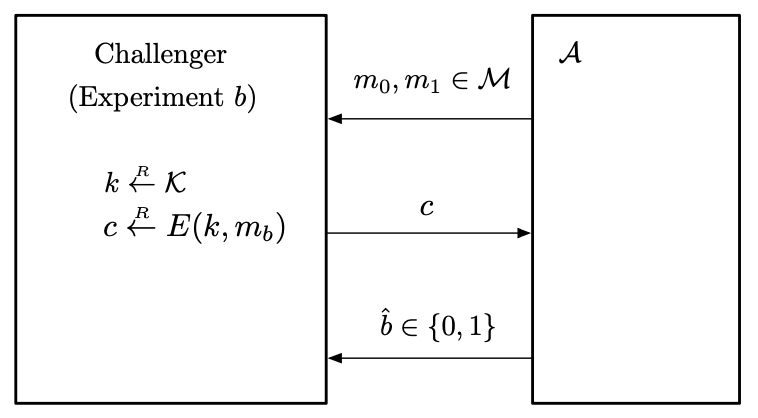
\includegraphics[width=0.5\linewidth]{figures/chapter2/fig1.png}
  \caption{攻击游戏 \ref{game:2-1} 中的实验 $b$}
  \label{fig:2-1}
\end{figure}

\begin{definition}[语义安全性]\label{def:2-2}
如果对于所有有效对手 $\mathcal{A}$,${\rm SS\mathsf{adv}}[\mathcal{A},\mathcal{E}]$ 的值都可以忽略不计,我们就称密码 $\mathcal{E}$ 是\textbf{语义安全}的。
\end{definition}

作为一个正式的定义,这还不是很完整,因为我们还没有定义``相同长度的消息"、``有效对手"和``可忽略不计"是什么意思。我们很快就会回到这个问题上。

让我们把这个正式定义与前面的讨论联系起来。假设攻击游戏 \ref{game:2-1} 中的对手 $\mathcal{A}$ 是确定性的。首先,对手以一种确定性的方式计算出消息 $m_0$和$m_1$,然后考察密文 $c$ 上的谓词 $\phi$,如果结果为真就输出 $1$,为假则输出 $0$。语义安全的意思是,式 \ref{eq:2-4} 中的 $\epsilon$ 是可以忽略不计的。如果 $\mathcal{A}$ 是概率性的,我们可以将 $\mathcal{A}$ 看作是这样的结构:它从某个适当的集合中生成一个随机数 $r$,并确定性地计算取决于$r$的消息 $m^{(r)}_0$ 和 $m^{(r)}_1$,接着评估谓词 $\phi^{(r)}$,它也取决于 $r$。这里,语义安全说明,当用 $m^{(r)}_0$、$m^{(r)}_1$ 和 $\phi^{(r)}$ 替换式 \ref{eq:2-4} 中的 $m_0$、$m_1$ 和 $\phi$ 时,$\epsilon$ 的大小仍然是可以忽略不计的,但现在的概率是针对一个随机选择的密钥和随机选择的 $r$ 值而言的。

\begin{remark}
现在让我们说一下,为什么我们要求在攻击游戏 \ref{game:2-1} 中,对手 $\mathcal{A}$ 计算出来的消息 $m_0$ 和 $m_1$ 必须是相同长度的。
\begin{itemize}
	\item 首先,消息的``长度"概念是针对特定的消息空间 $\mathcal{M}$ 而言的。换句话说,在指定一个消息空间时,我们必须指定一个规则,它能将长度(一个非负整数)与任何给定的消息关联起来。对于大多数具体的消息空间来说,这种联系是很显然的。例如,对于消息空间 $\{0, 1\}^{\leq L}$ (如例 \ref{exmp:2-2})来说,消息 $m\in\{0, 1\}^{\leq L}$ 的长度就是它的比特位数 $|m|$。然而,为了使我们的定义具有一定的普遍性,我们把长度的概念作为一个抽象概念。事实上,有些消息空间可能没有特别的长度概念,在这种情况下,所有的消息都可以被看作是长度为 $0$ 的。
	\item 其次,要求 $m_0$ 和 $m_1$ 具有相同的长度,意味着对手不会因为能够有效地根据长度区分两条密文就被认为是破坏了系统。这就是我们的正式定义所捕捉到的概念,即消息的加密被允许泄露消息的长度(但不会泄露其他信息)。
		
	我们在例 \ref{exmp:2-5} 中已经讨论过,在某些应用中,泄露消息的长度可能会带来灾难性的后果。然而,由于这个问题没有通用的解决方案,大多数现实世界的加密方案(例如TLS)根本没有尝试去隐藏消息的长度。这可能会导致真正的攻击。例如,Chen 等人表明,加密消息的长度可以揭示用户提供给云应用程序的私人数据的大量信息。他们以一个在线报税系统为例,但也有其他工作表明这种类型的攻击同样适用于很多其他的系统。
\end{itemize}
\end{remark}

\begin{example}\label{exmp:2-9}
令 $\mathcal{E}$ 是一个确定性密码,且是完美安全的。那么很容易看出,对于任意对手 $\mathcal{A}$(无论是否有效),我们都有 ${\rm SS\mathsf{adv}}[\mathcal{A},\mathcal{E}]=0$。这几乎可以立即从定理 \ref{theo:2-3} 中得出(唯一稍微复杂的是,我们在攻击游戏 \ref{game:2-1} 中的对手 $\mathcal{A}$ 可能是概率性的,但这很容易处理)。特别是,$\mathcal{E}$ 是语义安全的。因此,如果 $\mathcal{E}$ 是一次性密码本(见例 \ref{exmp:2-1}),那么对于所有对手 $\mathcal{A}$,我们有 ${\rm SS\mathsf{adv}}[\mathcal{A},\mathcal{E}]=0$,因此一次性密码本是语义安全的。由于语义安全的定义对于变长的消息空间来说是比较宽容的,所以也很容易看出,如果$\mathcal{E}$是变长一次性密码本(见例 \ref{exmp:2-2}),那么对于所有对手 $\mathcal{A}$,${\rm SS\mathsf{adv}}[\mathcal{A},\mathcal{E}]=0$都成立,因此变长一次性密码本也是语义安全的。
\end{example}

关于``有效"和``可忽略不计"这两个词,我们还要多说几句。在下面的 \ref{sec:2-3} 节中,我们将填补其余的细节(这些细节可能会稍显乏味,而且实际上并不是很有启发性)。 直观地说,\emph{可忽略不计}的意思是小到``对所有实际用途来说都是零":想像一下 $2^{-100}$ 这样的数字,如果你在下一年自燃的概率是 $2^{-100}$,那么你就不会担心这种事件的发生。我们还使用下列术语:
\begin{itemize}
	\item 一个\emph{有效对手}是一个能在``合理"时间内运行的对手。
	\item 如果 ${1}/{N}$ 可以忽略不计,就称$N$是\emph{超多项式(super-poly)}的。
	\item 一个\emph{多项式边界(poly-bounded)}的值是一个``合理"大小的数字。特别地,我们可以说,一个有效对手的运行时间是多项式边界的。
\end{itemize}

\begin{fact}\label{fact:2-6}
如果 $\epsilon$ 和 $\epsilon'$ 是两个可以忽略不计的值,而 $Q$ 和 $Q'$ 是两个多项式边界的值,那么:
\begin{enumerate}[(i)]
	\item $\epsilon+\epsilon'$ 是一个可以忽略不计的值,
	\item $Q + Q'$ 和 $Q\cdot Q'$ 都是多项式边界的,且
	\item $Q\cdot\epsilon$ 是一个可以忽略不计的值。
\end{enumerate}
\end{fact}



现在,读者可以把这些事实作为公理。我们不纠缠于这些技术问题,而是讨论一个例子,说明在分析一个使用语义安全密码的更大系统的安全性时,我们通常如何\emph{使用}这个定义。

\subsection{与较弱的安全概念的联系}\label{subsec:2-2-3}

\subsubsection{消息恢复攻击}\label{subsubsec:2-2-3-1}

直观地说,在消息恢复攻击(message recovery attack)中,对手被给定一个随机消息的加密,并且能够以明显优于随机猜测的概率(即概率为 ${1}/{|\mathcal{M}|}$)从密文中恢复消息。当然,任何合理的安全概念都应该排除这种攻击,语义安全当然也是如此。

虽然这在直觉上似乎是显而易见的,但我们给出了这一点的正式证明。我们这样做的动机之一是为了详细说明\emph{安全归约(security reduction)}的概念,这是用于推理系统安全性的主要技术。基本上,该证明将论证,任何能够有效地对 $\mathcal{E}$ 发起消息恢复攻击的有效对手 $\mathcal{A}$,都可以被用于建立一个能够破坏 $\mathcal{E}$ 的语义安全性的有效对手 $\mathcal{B}$;由于语义安全性意味着不存在这样的 $\mathcal{B}$,我们就可以得出结论,这样的 $\mathcal{A}$也是不存在的。

为了更详细地给出这个证明,我们需要一个消息恢复攻击的正式定义。和以前一样,这也是通过一个攻击游戏来完成的,该攻击游戏是一个挑战者与一个对手之间的游戏。

\begin{game}[消息恢复]\label{game:2-2}
给定一个定义在 $(\mathcal{K},\mathcal{M},\mathcal{C})$ 上的密码 $\mathcal{E}=(E,D)$,对于一个给定对手 $\mathcal{A}$,攻击游戏的过程如下:
\begin{itemize}
	\item 挑战者计算 $m\overset{\rm R}\leftarrow\mathcal{M}$,$k\overset{\rm R}\leftarrow\mathcal{K}$,$c\overset{\rm R}\leftarrow E(k,m)$,并将 $c$ 发送给对手。
	\item 对手输出一条消息 $\hat m\in\mathcal{M}$。
\end{itemize}
令 $W$ 为 $\hat m=m$ 成立的事件。我们称,在这种情况下,$\mathcal{A}$ 赢得该游戏。我们将对手 $\mathcal{A}$ 相对于 $\mathcal{E}$ 的\textbf{消息恢复优势}定义为:
$$
{\rm MR\mathsf{adv}}[\mathcal{A},\mathcal{E}]:=|\Pr[W] -{1}/{|\mathcal{M}|}|
$$
\end{game}

\begin{definition}[针对消息恢复的安全性]
如果对于所有有效对手 $\mathcal{A}$,${\rm MR\mathsf{adv}}[\mathcal{A},\mathcal{E}]$ 的值都可以忽略不计,我们就说密码 $\mathcal{E}$ \textbf{对消息恢复是安全的}。
\end{definition}

\begin{theorem}\label{theo:2-7}
令 $\mathcal{E}=(E,D)$ 是一个定义在 $(\mathcal{K},\mathcal{M},\mathcal{C})$ 上的密码。如果 $\mathcal{E}$ 是语义安全的,那么 $\mathcal{E}$ 对消息恢复也是安全的。
\end{theorem}

\begin{proof}
假设 $\mathcal{E}$ 是语义安全的。我们的目标是证明 $\mathcal{E}$ 对于消息恢复也是安全的。

为了证明 $\mathcal{E}$ 对于消息恢复是安全的,我们必须证明每一个有效对手 $\mathcal{A}$ 在攻击游戏 \ref{game:2-2} 中的优势都可忽略不计。为了证明这一点,我们给定一个任意但高效的对手 $\mathcal{A}$,现在我们的目标是证明 $\mathcal{A}$ 的消息恢复优势 ${\rm MR\mathsf{adv}}[\mathcal{A},\mathcal{E}]$ 是可以忽略不计的。令 $p$ 为 $\mathcal{A}$ 赢得消息恢复游戏的概率,那么有:
$$
{\rm MR\mathsf{adv}}[\mathcal{A},\mathcal{E}]=\left|p-{1}/{|\mathcal{M}|}\right|
$$
我们下面展示如何构建一个有效对手 $\mathcal{B}$,其在攻击游戏 \ref{game:2-1} 中的语义安全优势与 $\mathcal{A}$ 在攻击游戏 \ref{game:2-2} 中的消息恢复优势有如下关系:
\begin{equation}\label{eq:2-5}
{\rm MR\mathsf{adv}}[\mathcal{A},\mathcal{E}]\leq{\rm SS\mathsf{adv}}[\mathcal{B},\mathcal{E}]
\end{equation}
由于 $\mathcal{B}$ 是有效的,且我们假设 $\mathcal{E}$ 是语义安全的,因此式 \ref{eq:2-5} 中不等号右侧的值可以忽略不计,由此我们可以得出结论:${\rm MR\mathsf{adv}}[\mathcal{A},\mathcal{E}]$ 也可以忽略不计。

因此,完成证明所剩下的工作就是说明如何构造一个满足式 \ref{eq:2-5} 要求的有效的 $\mathcal{B}$。我们的想法是把 $\mathcal{A}$ 作为一个``黑箱",因为我们根本不需要了解 $\mathcal{A}$ 的内部运作情况。

以下是 $\mathcal{B}$ 的工作方式。对手 $\mathcal{B}$ 产生两条随机消息 $m_0,m_1\in\mathcal{M}$,并将其发送给自己的语义安全挑战者。这个挑战者向 $\mathcal{B}$ 发送一条密文 $c$,$\mathcal{B}$ 将其转发给 $\mathcal{A}$,\emph{就像它来自 $\mathcal{A}$ 的消息恢复挑战者一样}。当 $\mathcal{A}$ 输出一个信息 $\hat m$ 时,如果 $\hat m=m_1$,我们的对手 $\mathcal{B}$ 就输出 $\hat b=1$,否则输出 $\hat b=0$。

这就完成了对 $\mathcal{B}$ 的描述。注意,$\mathcal{B}$ 的运行时间与 $\mathcal{A}$ 的运行时间基本相同。我们现在分析 $\mathcal{B}$ 的语义安全优势,并将其与 $\mathcal{A}$ 的消息恢复优势关联起来。

对于 $b=0,1$,令 $p_b$ 表示当 $\mathcal{B}$ 的语义安全挑战者加密了 $m_b$ 时,$\mathcal{B}$ 的输出为 $1$ 的概率。根据定义,我们有:
$$
{\rm SS\mathsf{adv}}[\mathcal{B},\mathcal{E}]=|p_1-p_0|
$$
一方面,当 $c$ 是对 $m_1$ 的加密时,概率 $p_1$ 正好等于 $\mathcal{A}$ 在消息恢复游戏中获胜的概率,所以 $p_1=p$。另一方面,当 $c$ 是对 $m_0$ 的加密时,对手 $\mathcal{A}$ 的输出与 $m_1$ 无关,所以有$p_0={1}/{|\mathcal M|}$。由此可见:
$$
{\rm SS\mathsf{adv}}[\mathcal{B},\mathcal{E}]=|p_1-p_0|=|p-{1}/{|\mathcal{M}|}|={\rm MR\mathsf{adv}}[\mathcal{A},\mathcal{E}]
$$
这就证明了式 \ref{eq:2-5}。事实上,式 \ref{eq:2-5} 中的等号是成立的,但这对本证明并不重要。
\end{proof}

读者应该确保自己理解这个证明的逻辑,因为这种类型的证明将在本书中反复使用。我们再回顾一下该证明的重要部分,并给出另一种思考方式。

证明的核心建立在以下事实上:对于每一个在攻击游戏 \ref{game:2-2} 中攻击 $\mathcal{E}$ 的有效消息恢复对手 $\mathcal{A}$ ,都存在一个在攻击游戏 \ref{game:2-1} 中攻击 $\mathcal{E}$ 的有效语义安全对手 $\mathcal{B}$,使得:
\begin{equation}\label{eq:2-6}
{\rm MR\mathsf{adv}}[\mathcal{A},\mathcal{E}]\leq{\rm SS\mathsf{adv}}[\mathcal{B},\mathcal{E}]
\end{equation}
我们试图证明,如果 $\mathcal{E}$ 是语义安全的,那么 $\mathcal{E}$ 对消息恢复也是安全的。在上面的证明中,我们认为如果 $\mathcal{E}$ 是语义安全的,那么式 \ref{eq:2-6} 的右手边一定是可以忽略的,因此式 \ref{eq:2-6} 的右手边也一定是可以忽略的;由于这对所有有效对手 $\mathcal{A}$ 都是成立的,我们就能得出结论:$\mathcal{E}$ 对消息恢复是安全的。

证明该定理的另一种方法是反证法:如果 $\mathcal{E}$ 对消息恢复不是安全的,那么 $\mathcal{E}$ 也不是语义安全的。因此,我们假设 $\mathcal{E}$ 对消息恢复不安全。这意味着存在一个有效对手 $\mathcal{A}$,其消息恢复优势是不可忽略不计的。利用 $\mathcal{A}$,我们建立一个满足式 \ref{eq:2-6} 的有效对手 $\mathcal{B}$。根据假设,${\rm MR\mathsf{adv}}[\mathcal{A},\mathcal{E}]$ 是不可忽略不计的,而式 \ref{eq:2-6} 意味着 ${\rm SS\mathsf{adv}}[\mathcal{B},\mathcal{E}]$ 也只能是不可忽略的。由此,我们得出结论,$\mathcal{E}$ 不是语义安全的。

说得更简单些:为了证明语义安全意味着针对消息恢复的安全,我们展示了如何将一个可以打破消息恢复的有效对手转化成一个可以打破语义安全性的有效对手。

我们还强调,证明中构建的对手 $\mathcal{B}$ 只是将 $\mathcal{A}$ 作为一个``黑箱"。事实上,我们之后将要看到的几乎所有构造都是这种类型的。$\mathcal{B}$ 本质上只是 $\mathcal{A}$ 的一个包装,它由 $\mathcal{B}$ 的挑战者和 $\mathcal{A}$ 的单个运行实例之间的一些简单有效的``接口层"组成。理想情况下,我们希望接口层的计算复杂性不依赖于 $\mathcal{A}$ 的计算复杂性;然而,一些依赖性是不可避免的:如果一个攻击游戏允许 $\mathcal{A}$ 向其挑战者进行多次查询,$\mathcal{A}$ 的查询次数越多,接口层必须执行的工作就越多,但这个工作应该只依赖于查询的数量,而不是 $\mathcal{A}$ 的运行时间。

因此,当对手 $\mathcal{B}$ 可以像上述那样被结构化为与 $\mathcal{A}$ 互动的有效接口时,我们就称它是一个围绕对手 $\mathcal{A}$ 的\textbf{基本包装器(elementary wrapper)}。其突出的特性是:
\begin{itemize}
	\item 如果 $\mathcal{B}$ 是一个围绕 $\mathcal{A}$ 的基本包装器,并且 $\mathcal{A}$ 是有效的,那么 $\mathcal{B}$ 也是有效的。
	\item 如果 $\mathcal{C}$ 是一个围绕 $\mathcal{B}$ 的基本包装器,而 $\mathcal{B}$ 是 $\mathcal{A}$ 的一个基本包装器,那么 $\mathcal{C}$ 也是一个 $\mathcal{A}$ 的基本包装器。
\end{itemize}

\subsubsection{计算消息的单个比特}

如果一个加密方案是安全的,我们不仅应该很难恢复整个消息,也应该很难计算出关于消息的任何部分的信息。

我们不会在这里证明一个完全通用的定理,而是考虑一个具体的例子。

假设 $\mathcal{E}=(E,D)$ 是一个定义在 $(\mathcal{K},\mathcal{M},\mathcal{C})$ 上的密码,其中 $\mathcal{M}=\{0,1\}^L$。对于 $m\in\mathcal{M}$,如果 $m$ 中比特 $1$ 的数量是奇数,我们就定义 ${\rm parity}(m)$ 为的值 $1$,否则为 $0$。与这个结论等价的另一个结论是,${\rm parity}(m)$ 的值就等于对构成 $m$ 的所有比特做异或操作的结果。

我们将证明,如果 $\mathcal{E}$ 是语义安全的,那么给定一个随机消息 $m$ 的加密 $c$,很难预测 ${\rm parity}(m)$。由于 ${\rm parity}(m)$ 是一个 $1$ 比特的信息,任何对手都可以通过随机猜测以 ${1}/{2}$ 的概率猜中这个值。尽管如此,我们想要说明的是,没有任何有效对手能够稍微提升哪怕一点猜中的概率。

作为热身,假设有一个有效对手 $\mathcal{A}$ 能够以 $1$ 的概率猜中 ${\rm parity}(m)$。这意味着,对于每个消息 $m$,每个密钥 $k$,以及 $m$ 的每个加密 $c$,当我们向 $\mathcal{A}$ 提供密文 $c$ 时,它就能够输出 $m$ 的奇偶性。我们的对手任意选择两条消息 $m_0$ 和 $m_1$,但 ${\rm parity}(m_0)=0$,${\rm parity}(m_1)=1$。然后,它把这两条消息交给自己的语义安全挑战者,得到一个密文 $c$,然后将其转发给 $\mathcal{A}$。在收到 $c$ 后,对手 $\mathcal{A}$ 输出一个比特 $\hat b$,而 $\mathcal{B}$ 输出这个相同的比特 $\hat b$ 作为它自己的输出。很容易看出,$\mathcal{B}$ 的语义安全优势恰好是 $1$:当它的语义安全挑战者加密的是 $m_0$ 时,它总是输出 $0$,而当它的语义安全挑战者加密的是 $m_1$ 时,它总是输出 $1$。

这表明,如果 $\mathcal{E}$ 是语义安全的,就不存在能以 $1$ 的概率预测奇偶性的有效对手。然而,我们可以再进一步:如果 $\mathcal{E}$ 是语义安全的,就不存在能以明显优于 ${1}/{2}$ 的概率预测奇偶性的有效对手。为了准确说明这一点,我们给出一个攻击游戏。

\begin{game}[奇偶性预测]\label{game:2-3}
给定一个定义在 $(\mathcal{K},\mathcal{M},\mathcal{C})$ 上的密码 $\mathcal{E}=(E,D)$,对于一个给定对手 $\mathcal{A}$,攻击游戏的过程如下:
\begin{itemize}
	\item 挑战者计算 $m\overset{\rm R}\leftarrow\mathcal{M}$,$k\overset{\rm R}\leftarrow\mathcal{K}$,$c\overset{\rm R}\leftarrow E(k,m)$,并将 $c$ 发送给对手。
	\item 对手输出 $\hat b\in\{0,1\}$。
\end{itemize}

令 $W$ 为 $\hat b={\rm parity}(m)$ 的事件。我们定义 $\mathcal{A}$ 对于 $\mathcal{E}$ 的\textbf{奇偶性预测优势}为:
$$
{\rm Parity\mathsf{adv}}[\mathcal{A},\mathcal{E}]:=|\Pr[W]-{1}/{2}|
$$
\end{game}

\begin{definition}[奇偶性预测]
如果对于所有有效对手 $\mathcal{A}$,${\rm Parity\mathsf{adv}}[\mathcal{A},\mathcal{E}]$ 的值都可以忽略不计,我们就称密码 $\mathcal{E}$ \textbf{对奇偶性预测是安全的}。
\end{definition}

\begin{theorem}
令 $\mathcal{E}=(E,D)$ 是一个定义在 $(\mathcal{K},\mathcal{M},\mathcal{C})$ 上的密码,其中 $\mathcal{M}=\{0,1\}^L$。如果 $\mathcal{E}$ 是语义安全的,那么 $\mathcal{E}$ 对奇偶性预测是安全的。
\end{theorem}

\begin{proof}
与定理 \ref{theo:2-7} 的证明一样,我们也给出一个基于归约的证明。特别地,我们将证明,对于每个按照攻击游戏 \ref{game:2-3} 攻击 $\mathcal{E}$ 的奇偶性预测对手 $\mathcal{A}$,都存在一个按照攻击游戏 \ref{game:2-1} 攻击 $\mathcal{E}$ 的语义安全对手 $\mathcal{B}$,其中 $\mathcal{B}$ 是一个围绕 $\mathcal{A}$ 的基本包装器,满足:
$$
{\rm Parity\mathsf{adv}}[\mathcal{A},\mathcal{E}]=\frac{1}{2}\cdot{\rm SS\mathsf{adv}}[\mathcal{B},\mathcal{E}]
$$

令 $\mathcal{A}$ 是一个奇偶性预测对手,它能以 ${1}/{2}+\epsilon$ 的概率预测奇偶性,那么有 ${\rm Parity\mathsf{adv}}[\mathcal{A},\mathcal{E}]=\epsilon$。

下面我们展示,如何构建我们的语义安全对手 $\mathcal{B}$。

我们的对手 $\mathcal{B}$ 生成一个随机消息 $m_0$,并设置 $m_1\leftarrow m_0\oplus(0^{L-1}||1)$。也就是说,$m_1$ 除了最后一位被翻转之外,其他各位都与 $m_0$ 相同。因此 $m_0$ 与 $m_1$ 的奇偶性正好相反。

我们的对手 $\mathcal{B}$ 将这对 $m_0$,$m_1$ 发送给它自己的语义安全挑战者,并从挑战者那里收到一条密文 $c$,然后将 $c$ 转发给 $\mathcal{A}$。当 $\mathcal{A}$ 输出一个比特 $\hat b$ 时,如果 $\hat b={\rm parity}(m_0)$,我们的对手 $\mathcal{B}$ 就输出 $1$,否则就输出 $0$。

对于 $b=0,1$,令 $p_b$ 是当对手 $\mathcal{B}$ 的语义安全挑战者加密了 $m_b$ 的情况下对手 $\mathcal{B}$ 输出为 $1$ 的概率。所以根据定义,我们有:
$$
{\rm SS\mathsf{adv}}[\mathcal{B},\mathcal{E}]=|p_1-p_0|
$$

我们声称 $p_0={1}/{2}+\epsilon$,$p_1={1}/{2}-\epsilon$。这是因为,无论是加密的是 $m_0$ 还是 $m_1$,$m_b$ 在 $\mathcal{M}$ 上的分布都是均匀的,因此在 $b=0$ 的情况下,我们的奇偶性预测者 $\mathcal{A}$ 将以 ${1}/{2}+\epsilon$ 的概率输出 ${\rm parity}(m_0)$;而当 $b=1$ 时,我们的奇偶性预测者 $\mathcal{A}$ 将以 ${1}/{2}+\epsilon$ 的概率输出 ${\rm parity}(m_1)$,也就是以 $1-({1}/{2}+\epsilon)={1}/{2}-\epsilon$ 的概率输出 ${\rm parity}(m_0)$。

因此:
$$
{\rm SS\mathsf{adv}}[\mathcal{B},\mathcal{E}]=|p_1-p_0|=2|\epsilon|=2\cdot{\rm Parity\mathsf{adv}}[\mathcal{A},\mathcal{E}]
$$
这就证明了该定理。
\end{proof}

我们已经表明,如果一个对手能够有效地预测一条消息的奇偶性,那么它就可以被用来破坏语义安全。反过来说,事实证明,如果一个对手能够破坏语义安全,它就能有效地预测消息的某些谓词(见练习 3.15)。

\subsection{语义安全的结果}\label{subsec:2-2-4}

在本节中,我们将在一个具体的例子,即电子赌博的背景下研究语义安全的后果。这个例子的具体细节并不那么重要,但是这个例子说明了人们通常是如何在应用中使用语义安全假设的。

考虑下面这个极其简化的轮盘赌版本,它是一种在\emph{庄荷(house)}与一个\emph{玩家(player)}之间进行的游戏。玩家给庄荷 1 美元,然后它可以下两种赌注中的一种:
\begin{itemize}
	\item ``高或低",或者
	\item ``偶或奇"。
\end{itemize}
下注后,庄荷随机选择一个数字 $r\in\{0,1,...,36\}$。当 $r\neq 0$,并且:
\begin{itemize}
	\item 玩家下注``高",且 $r>18$,
	\item 玩家下注``低",且 $r\leq18$,
	\item 玩家下注``偶",且 $r$ 为偶数,
	\item 玩家下注``奇",且 $r$ 为奇数。
\end{itemize}
时,玩家获胜。如果玩家赢了,庄荷将付给它 2 美元(即玩家净赚 1 美元);如果玩家输了,庄荷将不会付给它钱(即玩家净输 1 美元)。显然,在这个游戏中,庄荷有一个虽然小但仍然显著的优势:玩家获胜的概率是 $18/37\approx48.65\%$。

现在,假设这个游戏是在互联网上进行的。此外,假设由于各种技术原因,在玩家下注\emph{之前},赌场需要公布 $r$ 的加密(也许是由一些与赌场共享密钥的监管机构来解密)。玩家可以在下注前自由地分析这个加密消息,以此试图来增加它赢钱的机会。然而,如果这个密码是好的,玩家的机会应该不能增加很多。让我们来证明这一点,假设 $r$ 是用定义在 $(\mathcal{K},\mathcal{M},\mathcal{C})$ 上的一个密码 $\mathcal{E}=(E,D)$ 加密的,其中 $\mathcal{M}=\{0,1,...,36\}$(在这个例子中,我们将 $\mathcal{M}$ 中的所有消息视为具有相同的长度)。另外,从现在开始,让我们称玩家为 $\mathcal{A}$,以强调玩家的对抗性,并假设 $\mathcal{A}$ 的策略可以被建模为一种有效算法。图 \ref{fig:2-2} 展示了这个游戏。这里,\emph{赌注(bet)}表示``高"、``低"、``偶"、``奇"中的一个。玩家 $\mathcal{A}$ 将赌注发送给庄荷,庄荷会评估函数 $W(r,bet)$。如果赌注相对于$r$而言是获胜的,函数的值就为$1$,否则就为$0$。我们定义:
$$
{\rm IR\mathsf{adv}}[A]:=|\Pr[W (r,bet)=1]-{18}/{37}|
$$

我们的目标是要证明以下定理。

\begin{figure}
  \centering
  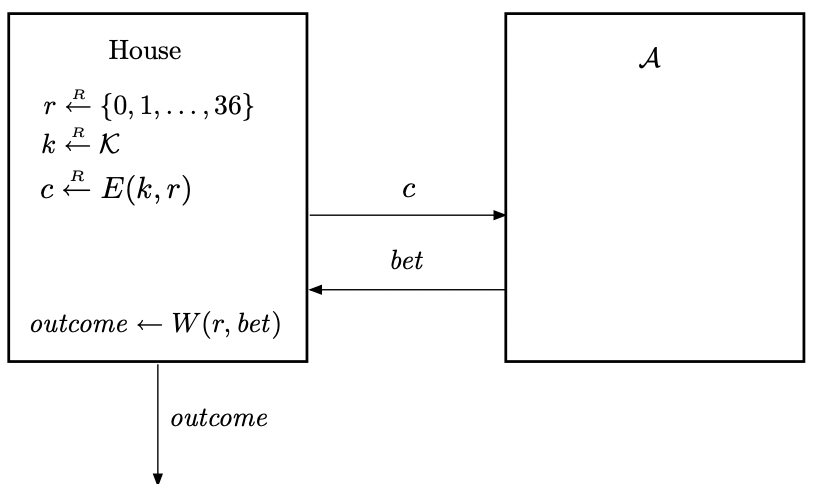
\includegraphics[width=0.6\linewidth]{figures/chapter2/fig2.png}
  \caption{网络轮盘赌}
  \label{fig:2-2}
\end{figure}

\begin{theorem}
如果 $\mathcal{E}$ 是语义安全的,那么对于每个有效玩家 $\mathcal{A}$,${\rm IR\mathsf{adv}}[\mathcal{A}]$ 的值都可忽略不计。
\end{theorem}

\begin{proof}
如我们在 \ref{subsec:2-2-3} 节所做的那样,我们仍然通过安全归约来证明这一点。更具体地说,我们将证明,对于每个玩家 $\mathcal{A}$,都存在一个语义安全对手 $\mathcal{B}$,使得 $\mathcal{B}$ 是 $\mathcal{A}$ 的一个基本包装器,并且:
\begin{equation}\label{eq:2-7}
{\rm IR\mathsf{adv}}[A]={\rm SS\mathsf{adv}}[\mathcal{B},\mathcal{E}]
\end{equation}

因此,如果存在一个优势不可忽略不计的有效玩家 $\mathcal{A}$,我们就能够得到一个有效的语义安全对手 $\mathcal{B}$,它可以打破 $\mathcal{E}$ 的语义安全性,而我们已经假设这是不可能的。因此,不存在这样的 $\mathcal{A}$。

为了分析我们的新对手 $\mathcal{B}$,我们先考虑一个``理想化"的互联网轮盘赌版本。在这个版本中,庄荷不公布实际的 $r$ 的加密,而是公布一个``假"值的加密,例如 $0$。图 \ref{fig:2-3} 展示了这个理想化的网络轮盘赌的逻辑。然而,请注意,在理想化版本的互联网轮盘赌中,庄荷仍然使用 $r$ 的实际值来决定游戏的结果。令 $p_0$ 为 $\mathcal{A}$ 在互联网轮盘赌中获胜的概率,$p_1$ 为 $\mathcal{A}$ 在理想化互联网轮盘赌中获胜的概率。

\begin{figure}
  \centering
  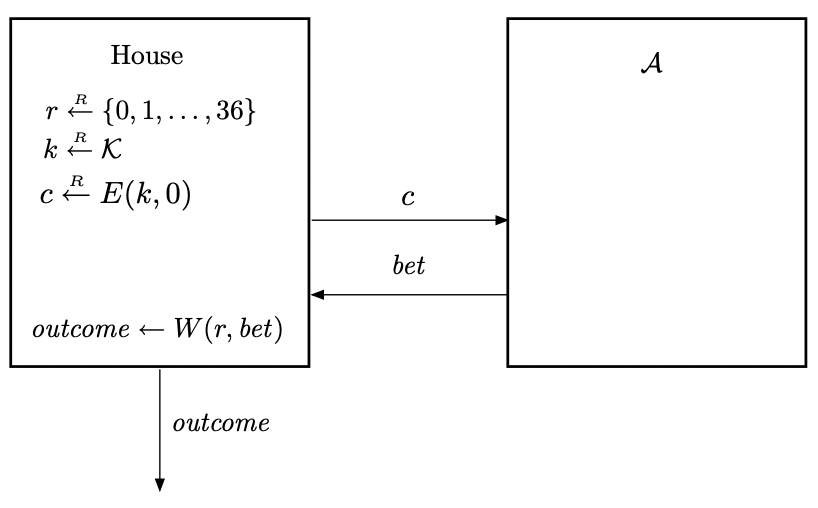
\includegraphics[width=0.6\linewidth]{figures/chapter2/fig3.png}
  \caption{网络轮盘赌的理想化版本}
  \label{fig:2-3}
\end{figure}

\begin{figure}
  \centering
  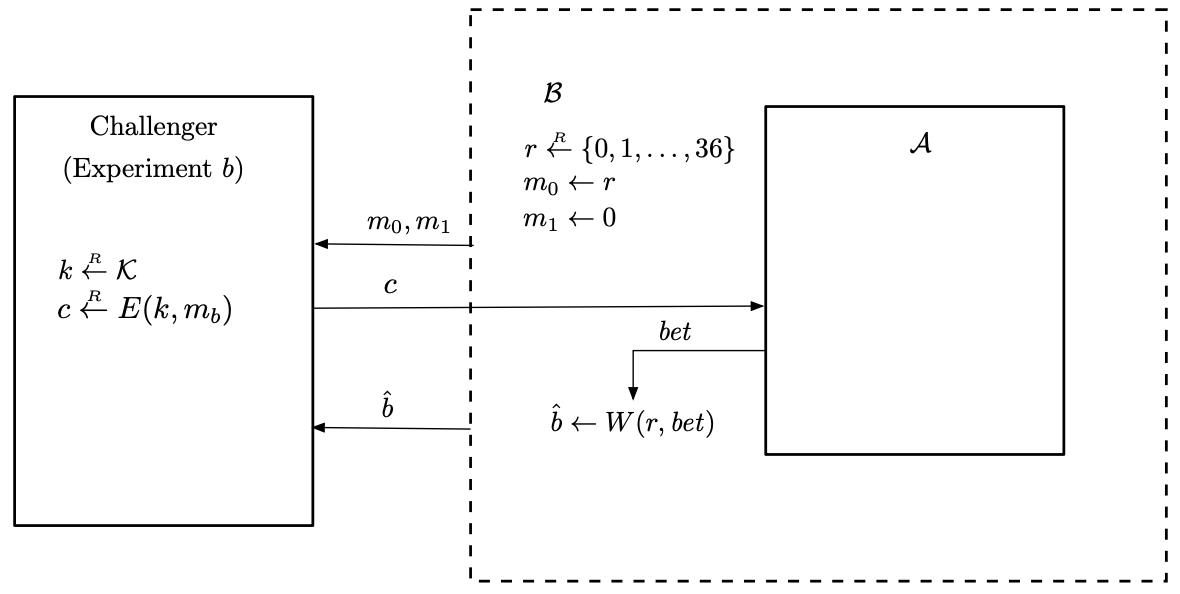
\includegraphics[width=0.85\linewidth]{figures/chapter2/fig4.png}
  \caption{攻击游戏 \ref{game:2-1} 中的语义安全对手 $\mathcal{B}$}
  \label{fig:2-4}
\end{figure}

我们的对手 $\mathcal{B}$ 被设计为在攻击游戏 \ref{game:2-1} 中进行游戏。因此,如果令 $\hat b$ 表示 $\mathcal{B}$ 在该游戏中的输出,我们有:
\begin{itemize}
	\item 如果 $\mathcal{B}$ 被置于实验 $0$ 中,那么有 $\Pr[\hat b=1]=p_0$;
	\item 如果 $\mathcal{B}$ 被置于实验 $1$ 中,那么有 $\Pr[\hat b=1]=p_1$。
\end{itemize}
图 \ref{fig:2-4} 展示了对手 $\mathcal{B}$ 的运行逻辑。通过构造可以看出,$\mathcal{B}$ 满足上面所声称的属性,特别是:
\begin{equation}\label{eq:2-8}
{\rm SS\mathsf{adv}}[\mathcal{B},\mathcal{E}]=|p_1-p_0|
\end{equation}

现在,考虑 $\mathcal{A}$ 在理想化互联网轮盘赌中获胜的概率 $p_1$。不管 $\mathcal{A}$ 的策略有多高明,它获胜的概率始终是 $18/37$,因为在这个理想化互联网轮盘赌中,\emph{赌注}的值是由 $c$ 计算出来的,而 $c$ 在统计上与 $r$ 的值毫无关系。因此:
\begin{equation}\label{eq:2-9}
{\rm IR\mathsf{adv}}[A]=|p_1-p_0|
\end{equation}

结合式 \ref{eq:2-8} 和式 \ref{eq:2-9},我们就能得到式 \ref{eq:2-7}。
\end{proof}

我们之后会反复使用这里用来分析互联网轮盘赌的方法。其基本思想是用一个理想化的系统组件替换原来的组件,然后分析这个新的、理想化版本的系统行为。

从上述例子中得到的另一个教训是,在推理一个系统的安全性时,我们将什么视为``对手",取决于我们想要做什么。在上面的分析中,我们用几个组件拼凑了一个新的对手 $\mathcal{B}$:其中一个组件是原来的对手 $\mathcal{A}$,而其他组件则是从系统的其他部分(在这个例子中是``庄荷"的算法)搜刮来的。这在我们全书的安全分析中会非常典型。直观地说,如果我们想象一个系统图,在安全分析的不同点上,我们将在系统的不同组件周围画一个圆圈,以确定我们在分析那个点时的``对手"。

\subsection{比特猜测:语义安全性的另一种表征}\label{subsec:2-2-5}

\ref{subsec:2-2-4} 小节中的例子很典型,它说明人们可以使用语义安全的定义来分析使用语义安全密码的较大系统的安全属性。然而,语义安全还有另一种更便于使用的表征,当我们试图证明一个给定的密码满足该定义时,它往往更方便使用。在这个替代性的表述中,我们定义一个新的攻击游戏。对手所扮演的角色与之前完全相同。然而,我们现在不再进行两个不同的实验,而是只有一个单一的实验。在这个\textbf{比特猜测版本(bit-guessing version)}的攻击游戏中,挑战者随机选择一个比特 $b\in\{0,1\}$并运行攻击游戏 \ref{game:2-1} 中的实验 $b$;对手的目标是以明显优于 ${1}/{2}$ 的概率猜中比特 $b$。下面是该攻击游戏的详细情况。

\begin{game}[语义安全性:比特猜测版本]\label{game:2-4}
给定一个定义在 $(\mathcal{K},\mathcal{M},\mathcal{C})$ 上的密码 $\mathcal{E}=(E,D)$,对于一个给定对手 $\mathcal{A}$,攻击游戏按如下方式运行:
\begin{itemize}
	\item 对手 $\mathcal{A}$ 计算相同长度的 $m_0, m_1\in\mathcal{M}$,并将它们发送给挑战者。
	\item 挑战者计算 $b\overset{\rm R}\leftarrow\{0,1\}$,$k\overset{\rm R}\leftarrow\mathcal{K}$,$c\overset{\rm R}\leftarrow E(k,m_b)$,并将 $c$ 发送给对手。
	\item 对手输出一个比特 $\hat b\in\{0,1\}$。
\end{itemize}

如果 $\hat b=b$,我们就称 $\mathcal{A}$ \textbf{赢得}这个游戏。
\end{game}

\begin{figure}
  \centering
  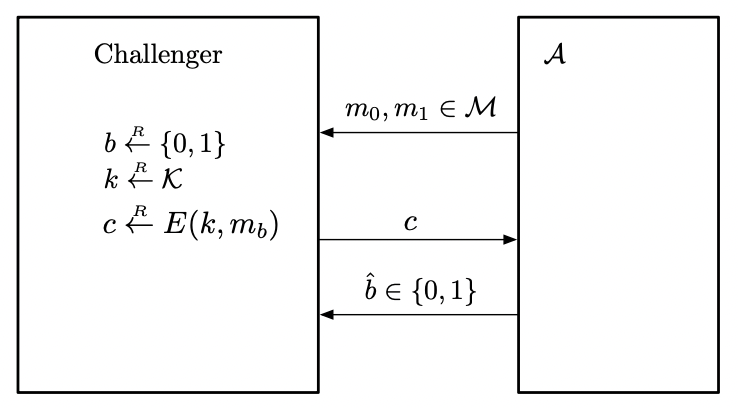
\includegraphics[width=0.5\linewidth]{figures/chapter2/fig5.png}
  \caption{攻击游戏 \ref{game:2-4}}
  \label{fig:2-5}
\end{figure}

图 \ref{fig:2-5} 展示了攻击游戏 \ref{game:2-4}。请注意,在这个游戏中,$\mathcal{A}$ 赢得游戏的事件是由 $b$ 与 $k$ 的随机选择、加密算法的随机选择(如果有的话)和对手的随机选择(如果有的话)共同构成的概率空间所定义的。

当然,任何对手都能以 ${1}/{2}$ 的概率赢得游戏,只需要完全忽略 $c$ 并随机选择 $\hat b$(或者说总是选择$\hat b=0$或总是选择$\hat b =1$)。我们感兴趣的是,对手能比随机猜测好多少。如果用 $W$ 表示对手赢得上述攻击游戏的比特猜测版本的事件,那么我们感兴趣的是 $|\Pr[W]-{1}/{2}|$ 的值,我们用 ${\rm SS\mathsf{adv}}^∗[\mathcal{A},\mathcal{E}]$ 表示该值。于是,我们有:

\begin{theorem}\label{theo:2-10}
对于每个密码 $\mathcal{E}$ 和每个对手 $\mathcal{A}$,我们都有:
\begin{equation}\label{eq:2-10}
{\rm SS\mathsf{adv}}[\mathcal{B},\mathcal{E}]= 2\cdot{\rm SS\mathsf{adv}}^∗[\mathcal{A},\mathcal{E}]
\end{equation}
\end{theorem}

\begin{proof}
这只是一个简单的计算。令 $p_0$ 是对手在攻击游戏 \ref{game:2-1} 的实验 $0$ 中输出 $1$ 的概率,$p_1$ 是对手在攻击游戏 \ref{game:2-1} 的实验 $1$ 中输出 $1$ 的概率。

现在考虑攻击游戏 \ref{game:2-4}。从现在开始,所有的事件和概率都是关于这个游戏的。如果我们以 $b=0$ 这一事件为条件,那么在这个条件概率空间中,挑战者和对手的所有其他随机选择的分布方式与攻击游戏 \ref{game:2-1} 的实验 $0$ 中的相应数值应该完全相同。因此,如果 $\hat b$ 是攻击游戏 \ref{game:2-4} 中对手的输出,则有:
$$
\Pr[\hat b=1\,|\,b=0]=p_0
$$
通过一个类似的论证,我们还可以得到:
$$
\Pr[\hat b=1\,|\,b=1]=p_1
$$
因此,我们有:
$$
\begin{aligned}
\Pr[\hat b=b]
&=\Pr[\hat b=b\,|\,b=0]\cdot\Pr[b=0]+\Pr[\hat b=b\,|\,b=1]\cdot\Pr[b=1]\\
&=\Pr[\hat b=0\,|\,b=0]\cdot \frac{1}{2}+\Pr[\hat b=b\,|\,b=1]\cdot\frac{1}{2}\\
& =\frac{1}{2}(1-\Pr[\hat b=1\,|\,b=0]+\Pr[\hat b=1\,|\,b=1])\\
& =\frac{1}{2}(1-p_0+p_1)
\end{aligned}
$$
因此:
$$
{\rm SS\mathsf{adv}}^∗[\mathcal{A},\mathcal{E}]=|\Pr[\hat b=b]-\frac{1}{2}|=\frac{1}{2}|p_1-p_0|=\frac{1}{2}\cdot{\rm SS\mathsf{adv}}[\mathcal{B},\mathcal{E}]
$$
这就证明了该定理。
\end{proof}

就像把 ${\rm SS\mathsf{adv}}[\mathcal{A},\mathcal{E}]$ 称为 $\mathcal{A}$ 的``语义安全优势"一样,我们将把 ${\rm SS\mathsf{adv}}^∗[\mathcal{A},\mathcal{E}]$ 称为 $\mathcal{A}$ 的``比特猜测语义安全优势"。

\subsubsection{一种推广}

事实证明,上面的情况是相当普遍的。虽然我们在本章中不需要它,但为了将来参考,我们在此指出如何推广上述情况到更一般的场景。我们可能会遇到一些情况,对于一些密码学系统(称为``$\mathcal{S}$"),其中的一些特定的安全属性(称为``$X$")可以用涉及两个实验(实验$0$和实验$1$)的攻击游戏来定义,其中对手 $\mathcal{A}$ 的协议在两个实验中是相同的,而挑战者的协议则是不同的。对于 $b=0,1$,我们定义 $W_b$ 为 $\mathcal{A}$ 在实验 $b$ 中输出为 $1$ 的事件,我们还定义:
$$
{\rm X\mathsf{adv}}[\mathcal{A},\mathcal{S}]:=|\Pr[W_0] -\Pr[W_1]|
$$
是 $\mathcal{A}$ 的 ``$X$ 优势"。就像上面一样,我们总是可以定义该攻击游戏的比特猜测版本,此时,挑战者随机选择一个 $b\in\{0,1\}$,然后运行实验 $b$ 作为它的协议。如果令 $W$ 是对手 $\mathcal{A}$ 的输出为 $b$ 的事件,那么我们定义:
$$
{\rm X\mathsf{adv}}^*[\mathcal{A},\mathcal{S}]:=|\Pr[W]-{1}/{2}|
$$
是 $\mathcal{A}$ 的``比特猜测$X$优势"。

使用与定理 \ref{theo:2-10} 的证明完全相同的计算方法,我们有:
\begin{equation}\label{eq:2-11}
{\rm X\mathsf{adv}}[\mathcal{A},\mathcal{S}]=2\cdot{\rm X\mathsf{adv}}^*[\mathcal{A},\mathcal{S}]
\end{equation}
\section{数学细节}\label{sec:2-3}

迄今为止,我们一直比较随意地使用\emph{有效(efficient)}和\emph{可忽略不计(negligible)}这两个术语,但没有给出它们的正式定义:
\begin{itemize}
	\item 我们要求,一个计算性密码要有\emph{有效}的加密和解密算法;
	\item 对于一个语义安全的密码,我们要求任何\emph{有效}对手在攻击游戏 \ref{game:2-1} 中的优势都\emph{可忽略不计}。
\end{itemize}
本节的目标是为这些术语提供精确的数学定义。虽然这些定义将密码学构建在坚实的数学理论基础上,并为我们的研究提供了一个令人满意的理论框架,我们仍需警告读者:
\begin{itemize}
	\item 这些定义相当复杂,需要大量的符号;并且
	\item 这些定义只是非常粗略地模拟了我们对这些术语的直观理解。
\end{itemize}
我们强调,读者可以安全地跳过这一节,而不会在理解上蒙受重大损失。在进入正式定义之前,我们先简要地告诉读者我们到底想要在这些定义中抓住哪些关键点:
\begin{itemize}
	\item 首先,当我们谈及一个有效的加密或解密算法时,我们通常指的是一种运行速度非常快的算法,比如说,以 $10$ 到 $100$ 个时钟周期每字节的速度加密数据。
	\item 其次,当我们谈及一个有效对手时,我们通常指的是一个能在某个大的,但仍然可行的时间(和其他计算资源)下完成运行的算法。通常情况下,我们假设一个试图破解密码学系统的对手愿意花费比密码学系统的使用者更多的资源。因此,$10,000$ 台计算机并行运行 $10$ 年,可以被视为一个有决心和耐心,且财力雄厚的对手的可行计算上限。然而,在某些情况下,比如在 \ref{subsec:2-2-4} 小节的网络轮盘赌的例子中,对手的计算时间可能会受到更大的限制。
	\item 第三,当我们说对手的优势可忽略不计时,我们的意思是,该优势是如此之小,以至于就所有实际目的而言,它都可以被视为等于零。正如我们在网络轮盘赌的例子中所看到的,如果在攻击游戏 \ref{game:2-1} 中,没有一个有效对手拥有超过 $2^{-100}$ 的优势,那么在实践中,也就没有一个玩家可以将它在网络轮盘赌中获胜的概率提升到 $2^{-100}$ 以上。
\end{itemize}

尽管我们对\emph{有效}一词的直观理解取决于上下文,但我们的正式定义不会做任何这种类型的区分。事实上,我们将采用计算复杂性理论的习惯,把\emph{有效}算法的概念等同于\emph{(概率性)多项式时间}算法的概念。无论好坏,这都为我们提供了一个独立于任何特定计算模型具体细节的形式化框架。

\subsection{可忽略不计、超多项式与多项式边界函数}\label{subsec:2-3-1}

我们首先从对\emph{可忽略不计(negligible)}、\emph{超多项式(super-poly)}和\emph{多项式边界(poly-bounded)}函数这三个概念的定义开始。

直观地讲,一个可忽略不计函数 $f:\mathbb{Z}_{\geq0}\to\mathbb{R}$ 是一个不仅在 $n\to\infty$ 时趋近于 $0$,而且趋近于 $0$ 的速度比任何多项式的倒数都要更快的函数。

\begin{definition}\label{def:2-5}
如果对于所有的 $c\in\mathbb{R}_{>0}$,都存在 $n_0\in\mathbb{Z}_{\geq 1}$ 使得对于所有的整数 $n\geq n_0$,都有 $|f(n)|<{1}/{n^c}$ 成立,我们就称函数 $f:\mathbb{Z}_{\geq1}\to\mathbb{R}$ 是\textbf{可忽略不计的(negligible)}。
\end{definition}

可忽略不计函数还有一种更加便于理解和使用的表示,如下所示:

\begin{theorem}\label{theo:2-11}
当且仅当对于所有的 $c>0$,都有:
\[
\lim_{n\to\infty}f(n)n^c=0
\]
时,函数 $f:\mathbb{Z}_{\geq1}\to\mathbb{R}$ 是可忽略不计的。
\end{theorem}

\begin{proof}
留作练习。
\end{proof}

\begin{example}\label{exmp:2-10}
一些不可忽略不计函数实例:
\[
2^{-n},
\quad
2^{-\sqrt{n}},
\quad
n^{-\log n}
\]
一些可忽略不计函数实例:
\[
\frac{1}{1000n^4+n^2\log n},
\quad
\frac{1}{n^{100}}
\]
\end{example}

当我们正式定义了``可忽略不计"这个术语后,定义``超多项式"就很容易了:

\begin{definition}\label{def:2-6}
如果 $1/f$ 可忽略不计,我们就称函数 $f:\mathbb{Z}_{\geq1}\to\mathbb{R}$ 是\textbf{超多项式的(super-poly)}。
\end{definition}

本质上,一个多项式边界函数 $f:\mathbb{Z}_{\geq1}\to\mathbb{R}$ 是一个被某个多项式(的绝对值)约束的函数。严格地说:

\begin{definition}\label{def:2-7}
如果存在 $c,d\in\mathbb{R}_{>0}$ 使得对于所有的整数 $n\geq0$,都有 $|f(n)|\leq n^c+d$,我们就称函数 $f:\mathbb{Z}_{\geq1}\to\mathbb{R}$ 是\textbf{多项式边界的(poly-bounded)}。
\end{definition}

请注意,如果 $f$ 是一个多项式边界函数,$1/f$ 就必然\emph{不是}一个可忽略不计函数。然而,正如下面的例子所说明的那样,请务必注意不要得出错误的推论。

\begin{example}\label{exmp:2-11}
定义 $f:\mathbb{Z}_{\geq1}\to\mathbb{R}$,使得对于所有偶数 $n$,都有 $f(n)={1}/{n}$;对于所有奇数 $n$,都有 $f(n)=2^{-n}$。那么 $f$ 不可忽略不计,但 $1/f$ 既不是多项式边界的,也不是超多项式的。
\end{example}

\subsection{计算性密码:正式定义}\label{subsec:2-3-2}

现在,我们讨论形式化的定义。首先,我们承认,我们之前说了个谎:当我们说一个计算性密码 $\mathcal{E}=(E,D)$ 定义在 $(\mathcal{K},\mathcal{M},\mathcal{C})$ 上,其中 $\mathcal{K}$ 是密钥空间,$\mathcal{M}$ 是消息空间,$\mathcal{C}$ 是密文空间,而且上述每个空间都是有限集时,我们并没有完全说出事实。在数学模型中(尽管在现实世界的系统中并不总是如此),我们将一个密码\emph{族} $\mathcal{E}$ 的密钥、消息和密文空间相关联,其索引为:
\begin{itemize}
	\item 一个\textbf{安全参数(security parameter)},它是一个正整数,用 $\lambda$ 表示,以及
	\item 一个\textbf{系统参数(system parameter)},它是一个比特序列,用 $\Lambda$ 表示。
\end{itemize}
因此,现在 $\mathcal{K},\mathcal{M},\mathcal{C}$ 不再单是三个有限集,而是三个有限集族:
\[
\{\mathcal{K}_{\lambda,\Lambda}\}_{\lambda,\Lambda},\quad
\{\mathcal{M}_{\lambda,\Lambda}\}_{\lambda,\Lambda},\quad
\{\mathcal{C}_{\lambda,\Lambda}\}_{\lambda,\Lambda}
\]
在本定义中,我们将其视为比特序列的集合(可以通过某些规范的编码函数来表示特定的数学对象)。

我们的想法是,当部署密码 $\mathcal{E}$ 时,安全参数 $\lambda$ 会被固定为某个值。一般来说,更大的 $\lambda$ 值往往意味着更高的安全水平(即针对拥有更多计算资源的对手的抵抗力),但这往往也意味着更长的密钥,以及更慢的加解密速度。因此,安全参数就像一个我们可以转动的``拨盘",用于在安全和效率之间设定一个权衡。

一旦选定了 $\lambda$,系统参数 $\Lambda$ 就会由一种特定于该密码的算法生成。我们的想法是,系统参数 $\Lambda$(连同 $\lambda$)给出了一种对密码的一个特定实例的详细描述,即:
\[
(\mathcal{K},\mathcal{M},\mathcal{C})
=(
\mathcal{K}_{\lambda,\Lambda},\;
\mathcal{M}_{\lambda,\Lambda},\;
\mathcal{C}_{\lambda,\Lambda}
)
\]
这一固定实例可能会被部署到一个更大的系统中,并被多方使用——$\lambda$ 和 $\Lambda$ 值都是公开的,(包括对手在内的)每个人都能知道。

\begin{example}\label{exmp:2-12}
考虑例 \ref{exmp:2-4} 中讨论的加性一次性密码本。该密码的描述中涉及到一个模数 $n$。要部署这样一个密码,需要生成一个合适的模数 $n$,并将其公开(有时甚至会将其直接``硬编码"到实现密码的程序里)。模数 $n$ 就是这个密码的系统参数。安全参数的特定值决定了 $n$ 的长度,以比特为单位。$n$ 本身可能由某些算法产生,这些算法可能是概率性的,其输出分布可能取决于预期的应用。例如,在某些场景下,我们可能希望 $n$ 是一个素数。
\end{example}

在进一步讨论之前,我们需要先定义有效算法的概念。在这个定义中,我们将只考虑以安全参数 $\lambda$ 和总长度由 $\lambda$ 的某个固定多项式约束的其他参数作为输入的算法 $A$。基本上,我们想称 $A$ 的运行时间以 $\lambda$ 的一个多项式为界,但如果 $A$ 是概率性的,情况将更加复杂:

\begin{definition}[有效算法]\label{def:2-8}
令 $A$ 是一个算法(可能是概率性的),它以一个安全参数 $\lambda\in\mathbb{Z}_{\geq1}$,以及其他被编码成的一个比特序列 $x\in\{0,1\}^{\leq p(\lambda)}$ 的若干参数作为输入,其中 $p$ 是某个固定的多项式。如果存在一个多项式边界函数 $t$ 和一个可忽略不计函数 $\epsilon$,使得对于所有的 $\lambda\in\mathbb{Z}_{\geq1}$ 和所有的 $x\in\{0,1\}^{\leq p(\lambda)}$,算法 $A$ 在输入 $(\lambda,x)$ 上的运行时间超过 $t(\lambda)$ 的概率最多为 $\epsilon(\lambda)$,我们就称 $A$ 为一个\textbf{有效算法(efficient algorithm)}。
\end{definition}

我们强调,上述定义中的概率是针对$A$的抛硬币而言的:对概率的这个约束必须对所有可能的输入$x$都成立。
\footnote{
\label{foot:2-1}
我们不坚持概率性算法在指定的时间范围内以$1$的概率停止,这样能给我们一点``回旋的余地",使得我们能够轻松地执行某些类型的随机抽样程序,这些程序没有\emph{先验的}运行时间限制,但不太可能运行非常长的时间(例如扔硬币直到出现正面)。另一种方法是约束\emph{预期的}运行时间,但由于技术原因,这被证明是有问题的。

请注意,这个有效算法的定义并不要求该算法在所有输入上都以$1$的概率停止。一个以$2^{-\lambda}$的概率进入无限循环的算法也可以满足这个定义,即使它不是以$1$的概率停止。这些问题是相当传统的。一般来说,我们只考虑在所有输入上都能以 $1$ 的概率停止的算法:这可以更自然地被看作是对算法的输出分布的要求,而不是对其运行时间的要求。
}

\vspace{5pt}

下面是一个正式定义,它抓住了由安全参数和系统参数进行参数化的系统的基本要求,并引入了更多的术语。在下面的定义中,我们用 ${\rm Supp}(P(\lambda))$ 来指代分布 $P(\lambda)$ 的\textbf{支持(support)},即算法 $P$ 在输入 $\lambda$ 上的所有可能输出的集合。

\begin{definition}\label{def:2-9}
一个\textbf{系统参数化(system parameterization)}是一个有效概率性算法 $P$,它以一个给定的安全参数 $\lambda\in\mathbb{Z}_{\geq1}$ 为输入,输出一个比特序列 $\Lambda$,称为\textbf{系统参数},其长度总是以 $\lambda$ 的一个多项式为界。我们还定义以下术语:
\begin{itemize}
	\item 对于一个由比特序列的有限集 $\mathbf{S}=\{\mathcal{S}_{\lambda,\Lambda}\}_{\lambda,\Lambda}$ 组成的集合,其中 $\lambda$ 在 $\mathbb{Z}_{\geq1}$ 上运行,$\Lambda$ 在 ${\rm Supp}(P(\lambda))$ 上运行,如果每个集合 $\mathcal{S}_{\lambda,\Lambda}$ 中所有比特序列的长度都以 $\lambda$ 的某个多项式 $p$ 为界,我们就称 $\mathbf{S}$ 为\textbf{具有系统参数化 $P$ 的空间族 (family of spaces with system parameterization $P$)}。
	\item 如果存在一个有效确定性算法,当输入 $\lambda\in\mathbb{Z}_{\geq1}$,$\Lambda\in{\rm Supp}(P(\lambda))$ 和 $s\in\{0,1\}^{\leq p(\lambda)}$ 时,能够确定 $s\in\mathcal{S}_{\lambda,\Lambda}$ 是否成立,我们就称 $\mathbf{S}$ 是\textbf{可有效识别的(efficiently recognizable)}。
	\item 如果存在一个有效概率性算法,当输入 $\lambda\in\mathbb{Z}_{\geq1}$ 和 $\Lambda\in{\rm Supp}(P(\lambda))$ 时,能够输出一个均匀分布在 $\mathcal{S}_{\lambda,\Lambda}$ 上的元素,我们就称 $\mathbf{S}$ 是\textbf{可有效采样的(efficiently sampleable)}。
	\item 如果存在一个有效确定性算法,当输入 $\lambda\in\mathbb{Z}_{\geq1}$,$\Lambda\in{\rm Supp}(P(\lambda))$ 和 $s\in\mathcal{S}_{\lambda,\Lambda}$ 时,能够输出一个非负整数,称为 $s$ 的\textbf{长度},我们就称 $\mathbf{S}$ \textbf{有一个有效长度函数(has an effective length function)}。
\end{itemize}
\end{definition}
现在,我们就可以为计算性密码给出一个完整、正式的定义:

\begin{definition}[计算性密码]\label{def:2-10}
一个\textbf{计算性密码}由一对算法 $E$ 和 $D$,以及三个具有系统参数化 $P$ 的空间族:
\[
\mathbf{K}=\{\mathcal{K}_{\lambda,\Lambda}\}_{\lambda,\Lambda},\quad
\mathbf{M}=\{\mathcal{M}_{\lambda,\Lambda}\}_{\lambda,\Lambda},\quad
\mathbf{C}=\{\mathcal{C}_{\lambda,\Lambda}\}_{\lambda,\Lambda}
\]
组成,满足:
\begin{enumerate}
	\item $\mathbf{K}$,$\mathbf{M}$和$\mathbf{C}$都是可有效识别的。
	\item $\mathbf{K}$是可有效采样的。
	\item $\mathbf{M}$有一个有效长度函数。
	\item 算法 $E$ 是一个有效概率性算法,它接受 $\lambda,\Lambda,k,m$ 作为输入,其中 $\lambda\in\mathbb{Z}_{\geq1}$,$\Lambda\in{\rm Supp}(P(\lambda))$,$k\in\mathcal{K}_{\lambda,\Lambda}$,$m\in\mathcal{M}_{\lambda,\Lambda}$,总是输出一个 $\mathcal{C}_{\lambda,\Lambda}$ 中的元素。
	\item 算法 $D$ 是一个有效确定性算法,它接受 $\lambda,\Lambda,k,c$ 作为输入,其中 $\lambda\in\mathbb{Z}_{\geq1}$,$\Lambda\in{\rm Supp}(P(\lambda))$,$k\in\mathcal{K}_{\lambda,\Lambda}$,$c\in\mathcal{C}_{\lambda,\Lambda}$,输出一个 $\mathcal{M}_{\lambda,\Lambda}$ 中的元素或一个特殊符号 $\mathsf{reject}\notin\mathcal{M}_{\lambda,\Lambda}$。
	\item 对于所有满足 $\lambda\in\mathbb{Z}_{\geq1}$,$\Lambda\in{\rm Supp}(P(\lambda))$,$k\in\mathcal{K}_{\lambda,\Lambda}$,$m\in\mathcal{M}_{\lambda,\Lambda}$ 和 $c\in{\rm Supp}(E(\lambda,\Lambda;k,m))$ 的 $\lambda,\Lambda,k,m,c$,我们都有 $D(\lambda,\Lambda;k,c)=m$。
\end{enumerate}
\end{definition}


注意,在上述定义中,加密和解密算法都接受 $\lambda$ 和 $\Lambda$ 作为辅助输入。为了与 \ref{subsec:2-2-1} 小节中所介绍的符号保持某种程度的一致性,我们将它们写成 $E(\lambda,\Lambda;\cdots)$ 和 $D(\lambda,\Lambda;\cdots)$。

\begin{example}\label{exmp:2-13}
考虑加性一次性密码本(见例 \ref{exmp:2-12})。在我们的正式框架中,安全参数 $\lambda$ 决定了模数 $n$ 的比特长度 $L(\lambda)$,也就是系统参数。系统参数生成算法将 $\lambda$ 作为输入,生成一个长度为 $L(\lambda)$ 的模数 $n$。函数 $L(\cdot)$ 应当是一个多项式边界函数。有了这个假设,很明显,系统参数生成算法满足我们对它的要求。对密钥、消息和密文空间的要求也得到了满足:
\begin{enumerate}
	\item 这些空间中的元素具有多项式边界长度:这是因为我们假设 $L(\cdot)$ 是一个多项式边界函数。
	\item 密钥空间是可有效采样的:只需随机选择 $k\overset{\rm R}\leftarrow\{0,\dots,n−1\}$ 即可。
	\item 密钥、信息和密文空间都是可有效识别的:只需测试一个比特序列 $s$ 是否是 $0$ 和 $n-1$ 之间的某个整数的二进制编码即可。
	\item 消息空间有一个有效长度函数:只需输出(比如说) $0$ 即可。
\end{enumerate}
\end{example}

我们注意到,有些密码(例如一次性密码本)可能根本就不需要系统参数。在这种情况下,我们可以假装系统参数是(比如说)一个空的字符序列。我们还注意到,有些密码也可能根本就没有真正的安全参数;事实上,很多行业标准的密码根本就是现成的,它们的密钥长度从最一开始就是固定的,也没有能够调整的安全参数。这在某些意义上是一种理论与实践的失配——但这就是现实。

这样,我们就完成了对计算性密码的正式数学描述,包含所有的细节。
\footnote{
请注意,我们在 \ref{subsec:2-2-1} 小节中对香农密码的定义不需要变动。我们在 \ref{subsec:2-2-1} 小节末尾声称的``任何确定性计算性密码都是香农密码"的说法需要恰当地理解:对于每个 $\lambda$ 和 $\Lambda$,我们都可以得到一个定义在 $(\mathcal{K}_{\lambda,\Lambda},\mathcal{M}_{\lambda,\Lambda},\mathcal{C}_{\lambda,\Lambda})$ 上的香农密码。
}
希望读者能够理解,虽然这些形式化的东西可以让我们在数学上给出精确并且有意义的陈述,但它们并不是很有启发性,而且在更多情况下甚至掩盖了真正发生的事情。因此,在正文中,我们将继续使用 \ref{subsec:2-2-1} 小节给出的简化术语与符号来讨论密码。但是读者需要理解,在本节讨论的所有形式化框架中,所有的陈述都有适当而自然的解释。这会是一个在接下来的章节中反复出现的模式:我们主要使用简化的术语来讨论各种类型的密码学方案,而不会考虑安全参数与系统参数。这些数学细节会在单独的小节中讨论,一般会遵循与这里所建立的通用模式相同的讨论方式。

\subsection{有效对手和攻击游戏}\label{subsec:2-3-3}

在定义语义安全性的概念时,我们必须定义所谓的\emph{有效对手 (efficient adversary)}是什么意思。由于这个概念将在本书中被广泛使用,我们要在这里提出一个更通用的框架。

对于任何类型的密码学方案,我们都需要使用一个攻击游戏来定义其安全性,它通常在一个对手 $\mathcal{A}$ 和一个挑战者之间进行:$\mathcal{A}$ 遵循一个任意的协议,而挑战者遵循某个简单且固定的协议,该协议由该密码学方案以及正在讨论的安全性概念决定。此外,对手和挑战者都将一个共同的安全参数 $\lambda$ 作为输入,挑战者通过计算出一个相应的系统参数 $\Lambda$,并将其发送给对手 $\mathcal{A}$ 来开始游戏。

为了对这些类型的交互进行建模,我们引入\textbf{交互式机器 (interactive machine)}的概念。在这样的机器 $M$ 启动之前,它总是会得到一个写在某个特殊的缓冲区中的安全参数 $\lambda$,然后将其内部状态的其他部分初始化为某些默认值。机器 $M$ 还有两个特殊的缓冲区:一个\emph{传入消息缓冲区(incoming message buffer)}和一个\emph{传出消息缓冲区(outcoming message buffer)}。机器 $M$ 可以被多次调用:当 $M$ 的外部环境向 $M$ 的传入消息缓冲区写入一个序列时,新的调用就开始了;$M$ 读取该消息,进行一些计算,更新其内部状态,并在其传出消息缓冲区上写入一个序列,结束调用,然后将传出消息交给外部环境。因此,$M$ 通过一个简单的消息传递系统与它的环境进行交互。我们假设 $M$ 可以在它的最后一个传出消息中嵌入某种信号以表示它已经停机,这样,$M$ 就会忽略任何在此之后调用它的尝试。

我们假设传入和传出机器 $M$ 的消息都被限制为\emph{恒定的长度}。这其实并不是一个真正的限制,因为我们总是可以通过发送许多较短的消息来模拟一个长消息的传输。然而,做出这样的限制可以简化一些技术问题。从现在开始,我们对对手和其他任何类型的交互式机器都施加这种长度限制。

对于任何给定的环境,我们可以通过计算 $M$ 在直至停机信号发出之前在所有调用中执行的步骤数来衡量 $M$ 的\textbf{总运行时间 (total running time)}。这个运行时间不仅取决于 $M$ 和它的随机选择,还取决于 $M$ 运行的环境。
\footnote{
与脚注 \ref{foot:2-1} 的讨论类似,我们对有效交互式机器的定义并不要求它在所有环境下都以 $1$ 的概率停机。这也是一个单独的问题,但它将是对我们考察的所有机器的一个隐式要求。
}

\begin{definition}[有效交互式机器]\label{def:2-11}
如果存在一个多项式边界函数 $t$ 和一个可忽略不计函数 $\epsilon$,使得对于所有环境(甚至不是计算上有界的环境),$M$ 的总运行时间超过 $t(\lambda)$ 的概率最多为 $\epsilon(\lambda)$,我们就称 $M$ 是一个\textbf{有效交互式机器 (efficient interactive machine)}。
\end{definition}

自然而然地,我们可以将对手建模为一个交互式机器。一个\textbf{有效对手 (efficient adversary)}就是一个有效交互式机器。

我们可以将两个交互式机器连接在一起,比如使用 $M'$ 和 $M$ 构建一个新的交互式机器 $M''=\langle M',M\rangle$。从环境到 $M''$ 的消息总是会被转发到 $M'$。机器 $M'$ 可以向环境发送消息,也可以向 $M$ 发送消息;在后一种情况下,$M$ 发送的输出消息会被发送到 $M'$。我们假设,如果 $M$ 停机,那么 $M'$ 就不会再向它发送任何消息。

因此,当 $M''$ 被调用时,其传入的消息会被转发到 $M'$,然后 $M'$ 和 $M$ 可能会交互若干次,然后,当 $M'$ 向环境发送消息时,$M''$ 的调用就结束了。我们将 $M'$ 称为``开放"机器(即它与外界交互),将 $M$ 称为``封闭"机器(即它只与 $M'$ 交互)。

\vspace{5pt} 

自然,我们可以通过将两台这样的机器像上面那样连接在一起,以模拟一个挑战者与一个对手之间的交互:挑战者被当作一台开放机器,而对手被当作一台封闭机器。

在我们的安全归约中,我们通常会展示如何使用能够破坏某个系统的对手 $\mathcal{A}$ 来构建能够破坏其他系统的对手 $\mathcal{B}$。我们想要的基本属性是,如果 $\mathcal{A}$ 是有效的,那么 $\mathcal{B}$ 也是如此。然而,我们的归约几乎总是采用一种非常特殊的形式,即 $\mathcal{B}$ 是一个围绕 $\mathcal{A}$ 的包装器,它由 $\mathcal{B}$ 的挑战者与 $\mathcal{A}$ 的单个运行实例之间的某个简单而有效的``接口层"组成。

理想情况下,我们希望接口层的计算复杂度不依赖于 $\mathcal{A}$ 的计算复杂度;然而,某种程度的依赖性是不可避免的:$\mathcal{A}$ 向其挑战者发起越多的查询,接口层就必须执行越多的工作。但是,这种工作应该只依赖于这种查询的数量,而不依赖于 $\mathcal{A}$ 的运行时间。

为了严格定义这一点,我们将 $\mathcal{B}$ 构建为一个组合式机器 $\langle M',M\rangle$,其中 $M'$ 代表接口层(即``开放"机器),$M$ 代表 $\mathcal{A}$ 的实例(即``封闭“机器)。这就将我们导向下面的定义。

\begin{definition}[基本包装器]\label{def:2-12}
如果存在一个多项式边界函数 $t$ 和一个可忽略不计函数 $\epsilon$,使得对于所有的 $M$(不必是计算上有界的),当我们在一个任意的环境(同样不必是计算上有界的)中执行组合式机器 $\langle M',M\rangle$ 时,下述属性成立:
\begin{quote}
在组合式机器 $\langle M',M\rangle$ 执行过程中的每一点上,如果 $I$ 是 $M'$ 和 $M$ 之间截至该点的交互次数,$T$ 是 $M'$ 截至该点的总运行时间,则 $T>t(\lambda+I)$ 成立的概率最大为 $\epsilon(\lambda)$。
\end{quote}
时,我们就称交互式机器 $M'$ 为一个\textbf{有效接口 (efficient interface)}。如果 $M'$ 是一个有效接口,而 $M$ 是任何机器,我们就称 $\langle M',M\rangle$ 是\textbf{一个围绕 $M$ 的基本包装器 (an elementary wrapper around $M$)}。
\end{definition}

因此,当对手 $\mathcal{B}$ 能够像上面那样被构造成一个与 $\mathcal{A}$ 交互的有效接口时,我们就称 $\mathcal{B}$ 是一个围绕 $\mathcal{A}$ 的基本包装器。我们的定义旨在设计一个适用于协同工作的形式,其突出的属性是:
\begin{itemize}
	\item 如果 $\mathcal{B}$ 是一个围绕 $\mathcal{A}$ 的基本包装器,而 $\mathcal{A}$ 是有效的,则 $\mathcal{B}$ 也是有效的。
	\item 如果 $\mathcal{C}$ 是一个围绕 $\mathcal{B}$ 的基本包装器,$\mathcal{B}$ 是一个围绕 $\mathcal{A}$ 的基本包装器,则 $\mathcal{C}$ 也是一个围绕 $\mathcal{A}$ 的基本包装器。
\end{itemize}

还要注意的是,在我们的攻击游戏中,挑战者通常满足我们对有效接口的定义。对于这样的挑战者和任何一个有效对手 $\mathcal{A}$,我们可以将它们的整个交互看作是一个单一的有效机器的交互。

\begin{snote}[查询有界的对手。]
在我们到目前为止所介绍的所有攻击游戏中,对手都只会发起固定数量的查询。在后面的章节中,我们将看到允许对手 $\mathcal{A}$ 进行多次查询的攻击游戏——即使对手允许发起的查询数量没有先验约束,但如果 $\mathcal{A}$ 是有效的,查询的次数也会被某个多项式边界值 $Q$ 所约束(至少以几乎可忽略不计的概率)。在证明这种攻击游戏的安全性时,为了基于 $\mathcal{A}$ 设计一个基本包装器 $\mathcal{B}$,我们通常会\emph{预先}向 $\mathcal{B}$ 告知 $\mathcal{A}$ 最终会发起查询的次数上界 $Q$。为了将其应用于我们的正式框架,我们可以这样设计:让 $\mathcal{A}$ 在一开始就发送一连串 $Q$ 个特殊消息,来向 $\mathcal{B}$ 发出这个查询次数上界的``信号"。如果这样做,那么 $\mathcal{B}$ 不仅可以在其逻辑中使用 $Q$ 值,而且还可以在不违反定义 \ref{def:2-12} 中的时间约束的情况下,在取决于 $Q$ 的时间内运行。这就使得 $\mathcal{B}$ 可以初始化一些大小可能取决于 $Q$ 的数据结构。当然,所有这些都只是一个理论上的``权宜之计",用来绕过那些本来就过于严苛的技术约束,因此不应该太过认真。我们在接下来的章节中都不会再明确说明这种``信号"机制。
\end{snote}


\subsection{语义安全性:正式定义}\label{subsec:2-3-4}

在定义任何类型的安全性时,我们都把对手在攻击游戏中的优势定义为一个函数 ${\rm Adv}(\lambda)$。它的值由攻击游戏中特定事件发生的概率来决定:对于 $\lambda$ 的每个值,我们都能得到一个不同的概率空间,它由挑战者的随机选择和对手的随机选择共同决定。安全性意味着,对于每个有效对手,函数 ${\rm Adv}(\cdot)$ 都是可忽略不计的。

下面,我们考察密码语义安全性这一具体的情况。在攻击游戏 \ref{game:2-1} 中,我们定义了 ${\rm SS\mathsf{adv}}[\mathcal{A},\mathcal{E}]$ 这个值。这个值实际上是安全参数 $\lambda$ 的一个函数。对定义 \ref{def:2-2} 的正确解释是,如果对于所有有效对手 $\mathcal{A}$(如上所述,它被建模为一个交互式机器)来说,安全参数 $\lambda$ 的函数 ${\rm SS\mathsf{adv}}[\mathcal{A},\mathcal{E}]$ 都可忽略不计(如定义 \ref{def:2-5} 所定义的那样),则 $\mathcal{E}$ 是安全的。回顾一下,挑战者和对手都接受 $\lambda$ 作为共同的输入。控制流从挑战者开始,它将系统参数发送给对手。对手随后将它的查询发送给挑战者,其中包含两条明文,而挑战者会用一条密文作为应答。最后,对手会输出一个比特(严格来说,在我们的形式化机器模型中,这个``输出"是发送给挑战者的一条消息,然后挑战者停机)。${\rm SS\mathsf{adv}}[\mathcal{A},\mathcal{E}](\lambda)$ 的值由挑战者的随机选择(包括系统参数的选择)和对手的随机选择共同决定。图 \ref{fig:2-6} 展示了攻击游戏 \ref{game:2-1} 的全貌。

\begin{figure}
	\centering
	\tikzset{every picture/.style={line width=0.75pt}}

\begin{tikzpicture}[x=0.75pt,y=0.75pt,yscale=-0.9,xscale=0.9]

\draw  [line width=1.2] (0,80) -- (180,80) -- (180,330) -- (0,330) -- cycle ;
\draw  [line width=1.2] (290,80) -- (410,80) -- (410,330) -- (290,330) -- cycle ;

\draw  [->]  (180,260) -- (290,260) ;
\draw  [->]  (290,220) -- (180,220) ;
\draw  [->]  (290,300) -- (180,300) ;
\draw  [->]  (180,180) -- (290,180) ;
\draw  [->]  (220,0) -- (220,40) -- (90,40) -- (90,80) ;
\draw  [->]  (220,0) -- (220,40) -- (350,40) -- (350,80) ;

\draw (90,100) node   [align=left] {挑战者};
\draw (90,125) node   [align=left] {(实验 $b$)};
\draw (32,220) node [anchor=west] [inner sep=0.75pt]    {$k\overset{\mathrm{R}}{\leftarrow }\mathcal{K}_{\lambda ,\Lambda }$};
\draw (32,250) node [anchor=west] [inner sep=0.75pt]    {$c\overset{\mathrm{R}}{\leftarrow } E( \lambda ,\Lambda ;k,m_{b})$};
\draw (235,256.6) node [anchor=south] [inner sep=0.75pt]   {$c$};
\draw (235,296.6) node [anchor=south] [inner sep=0.75pt]   {$\hat{b} \in \{0,1\}$};
\draw (235,216.6) node [anchor=south] [inner sep=0.75pt]   {$m_{0} ,m_{1} \in \mathcal{M}_{\lambda ,\Lambda }$};
\draw (350,100) node    {$\mathcal{A}$};
\draw (90,155) node    {$\Lambda \overset{\mathrm{R}}{\leftarrow } P( \lambda )$};
\draw (235,176.6) node [anchor=south] [inner sep=0.75pt]   {$\Lambda $};
\draw (222,20) node [anchor=west][inner sep=0.75pt]    {$\lambda $};

\end{tikzpicture}
	\caption{攻击游戏 \ref{game:2-1} 的完整详细版本}
	\label{fig:2-6}
\end{figure}

此外,在攻击游戏 \ref{game:2-1} 中,我们要求对手给出的两条消息具有相同的长度,这意味着定义 \ref{def:2-10} 第 3 部分给出的长度函数在两条消息上评估为相同的值。

根据这个形式上的定义,我们也可以讨论一下密码 $\mathcal{E}$ 的不安全性到底意味着什么。这意味着存在一个有效对手 $\mathcal{A}$,使得 ${\rm SS\mathsf{adv}}[\mathcal{A},\mathcal{E}]$ 是一个安全参数 $\lambda$ 的不可忽略不计函数。也就意味着,对于某个 $c>0$ 和无限多个安全参数 $\lambda$ 的取值,有 ${\rm SS\mathsf{adv}}[\mathcal{A},\mathcal{E}]\geq{1}/{\lambda^c}$ 成立。所以,不安全性并不意味着对手在所有安全参数 $\lambda$ 的取值情况下都能``攻破"密码 $\mathcal{E}$,而只是攻破密码 $\mathcal{E}$ 的安全参数取值有无限多个。

在正文中,我们一般会忽略安全参数、系统参数等。但读者需要明白,所有这些``简写"的背后都存在一个相应的精确的、形式化的数学表达。特别地,我们经常会称某个值 $v$ 是可忽略不计的(多项式边界的),这实际上意味着 $v$ 是安全参数的一个可忽略不计(多项式边界)函数。
\section{一个有趣的应用:匿名路由}\label{sec:2-4}

我们的老朋友 Alice 想向 Bob 发送一条消息 $m$,但她不想让 Bob 或其他人知道这条消息 $m$ 是来自 Alice 的。比如说,Bob 可能在经营一个公共论坛,而 Alice 想在论坛上匿名发布一条评论。匿名发帖可以让 Alice 在不表明自己的真实身份的前提下自由地讨论健康问题等敏感议题。在本节中,我们假设 Alice 只想在论坛上发布\emph{一条}消息。

一种方法是,Alice 选择一个代理,即 Carol,她将 $m$ 发送给 Carol,并让 Carol 将消息转发给 Bob。这显然不能为 Alice 提供匿名性,因为任何监测网络的人都能看到 $m$ 是由 Alice 发给 Carol,再由 Carol 发给 Bob 的。通过追踪 $m$ 在网络中的路径,任何人都可以看到这个帖子来自于 Alice。

一种更好的方法是,Alice 与 Carol 建立一个共享密钥 $k$,并向 Carol 发送 $c:=E(k,m)$,其中 $\mathcal{E}=(E,D)$ 是一个语义安全的密码。Carol 对 $c$ 进行解密,并将 $m$ 转发给 Bob。现在,监测网络的人将看到一条由 Alice 发给 Carol 的消息,以及另一条由 Carol 发给 Bob 的消息。然而,这种方法仍然不能确保 Alice 的匿名性:如果在某一天,Carol 收到的唯一消息就来自 Alice,而她发送的唯一消息是给 Bob 的,那么监测者就可以将这两者联系起来,仍然可以推断出发布的信息来自 Alice。

我们可以通过让 Carol 提供一个\emph{混合服务(mixing service)}来解决这个问题。所谓混合服务,就是将来自许多不同参与方$A_1,\dots,A_n$ 的消息进行混合的服务。对于$i=1,\dots,n$,Carol 与 $A_i$ 建立一个密钥 $k_i$,每个参与方 $A_i$ 都向 Carol 发送了一条加密消息 $c_i:=E(k_i,\,\langle destination_i,m_i\rangle)$。Carol 收集所有 $N$ 条传入的密文,用正确的密钥解密每条密文,并将得到的明文以某种随机的顺序转发到它们的目的地。现在,一个监测者在检查 Carol 的通信时,只能看到有 $n$ 条消息传入和 $n$ 条消息传出,但无法知道哪条消息被转发到了哪里。Alice 的消息是 Carol 发出的 $n$ 条消息中的某一条,但监测者无法知道到底是哪一条。我们说 Alice 的\emph{匿名集(anonymity set)}大小为 $n$。

剩下的问题是,Carol 仍然知道 Alice 是在论坛发布某条特定消息的人。为了消除这最后的风险,Alice 可以使用多个混合服务,比如说Carol 和 David。她与 Carol 建立一个密钥 $k_{\rm c}$,与 David 建立一个密钥 $k_{\rm d}$。为了向 Bob 发送她的消息,她按如下方式构建她的密文 $c_2$:
\begin{equation}\label{eq:2-12}
c_2:=E(k_{\rm c},E(k_{\rm d},m))
\end{equation}
完整起见,Alice 可能想在密文中嵌入路由信息,因此 c2 的实际构造为:
\[
c_2:=E(k_{\rm c},\,\langle\mathsf{David},c_1\rangle)\quad\text{where}\quad
c_1:=E(k_{\rm d},\,\langle\mathsf{Bob},m\rangle)
\]
接下来,Alice 将 $c_2$ 发送给 Carol。Carol 对 $c_2$ 进行解密并得到明文 $\langle\mathsf{David},c_1\rangle$,这示意她要把 $c_1$ 发送给 David。David 解密 $c_1$ 得到明文 $\langle\mathsf{Bob},m\rangle$,示意他把 $m$ 发送给 Bob。图 \ref{fig:2-7} 展示了这个解密嵌套密文的过程,它类似于一层一层地剥开洋葱。由于这个原因,这种路由过程通常被称为\emph{洋葱路由(onion routing)}。

\begin{figure}
  \centering
  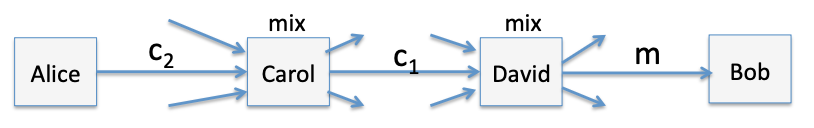
\includegraphics[width=0.6\linewidth]{figures/chapter2/fig7.png}
  \caption{一个使用两层混合的洋葱路由的例子}
  \label{fig:2-7}
\end{figure}

现在,即使 Carol 监测了所有的网络流量,也不能确定谁在 Bob 的论坛上发布了哪条消息。这对 David 来说也是如此。然而,如果 Carol 和 David 是串通的,他们就能搞清楚这些信息。由于这个原因,Alice 可能会通过两个以上的混合网络来传递她的信息。只要其中的一个混合服务不与其他混合服务共谋,Alice 就能够保护她的匿名性。

一个稍微有点复杂的情况是,当 Alice 与 David 建立共享秘钥 $k_{\rm d}$ 时,她不能向 David 透露她的身份。否则,David 就会知道 $c_1$ 来自 Alice,这是我们不希望看到的。这个目标并不难实现,我们将在本书后面介绍如何做到这一点(见 \ref{sec:21-13} 节)。

\begin{snote}[嵌套加密的安全性。]
为了保持Alice的匿名性,知道 $k_{\rm c}$ 的 Carol 不能从式 \ref{eq:2-12} 的嵌套密文 $c_2$ 中获取任何关于 $m$ 的信息。否则,Carol 就有可能利用她从 $c_2$ 中了解到的关于 $m$ 的信息,将 Alice 与她在 Bob 的论坛上发的帖子联系起来。比如说,假设 Carol 可以从 $c_2$ 中了解到 $m$ 的前几个字符,然后她发现 Bob 的论坛上只有一个帖子以这些字符开头。那么 Carol 就可以将整个帖子与 Alice 关联起来,因为她知道 $c_2$ 是来自 Alice 的。

对 David 来说也是如此:知道 $k_{\rm d}$ 的 David 最好无法从式 \ref{eq:2-12} 的嵌套密文 $c_2$ 中得知任何关于 $m$ 的信息。

我们下面论证,如果 $\mathcal{E}$ 是语义安全的,那么在给定 $c_2$ 和 $k_c$ 或 $k_d$ 两个密钥中的一个的情况下,任何有效对手都无法了解任何关于 $m$ 的信息。
\end{snote}

一般地,对于定义在 $(\mathcal{K},\mathcal{M},\mathcal{C})$ 上的密码 $\mathcal{E}=(E,D)$,我们定义 $n$ 层嵌套密码 $\mathcal{E}_n=(E_n,D_n)$ 如下:
\[
E_n\big((k0,\dots,k_{n-1}),\,m\big)=E\big(k_{n-1},E(k_{n-2},\,\cdots E(k_0,m)\cdots\big)
\]
解密算法以相反的顺序使用密钥:
\[
D_n\big((k0,\dots,k_{n-1}),\,c\big)=D\big(k_0,E(k_1,\,\cdots E(k_{n-1},m)\cdots\big)
\]
我们的目标是表明,如果$\mathcal{E}$是语义安全的,那么就算对手得到了除了$k_0,\dots,k_{n-1}$中某一个以外的所有密钥,$\mathcal{E}_n$也是语义安全的。为了更加精确,我们定义两个实验:实验$0$和实验$1$,对于$b=0,1$,实验$b$的工作方式如下:
\begin{itemize}
	\item 对手将 $(m_0,m_1,d)$ 交给挑战者,其中 $m_0,m_1\in\mathcal{M}$ 是长度相等的两条消息,且 $0\leq d<n$。
	\item 挑战者选择 $n$ 个密钥 $k_0,\dots,k_{n-1}\overset{\rm R}\leftarrow\mathcal{K}$ 并计算 $c\overset{\rm R}\leftarrow E_n\big((k_0,\dots,k_{n-1}),\,m_b\big)$。它将 $c$ 和所有的密钥 $k_0,\dots,k_{n-1}$ 一起发送给对手,但不包括密钥 $k_{\rm d}$。
	\item 对手输出一个比特 $\hat b\in\{0,1\}$。
\end{itemize}
这个游戏抓住了这样一个事实:对手得到除 $k_{\rm d}$ 以外的所有密钥 $k_0,\dots,k_{n-1}$,并试图破坏语义安全性。

如同语义安全性的定义,我们定义对手的优势 $\mathrm{NE^{(n)}}\mathsf{adv}[\mathcal{A},\mathcal{E}]$ 如下:
\[
\mathrm{NE^{(n)}}\mathsf{adv}[\mathcal{A},\mathcal{E}]=\big\vert\Pr[W_0]-\Pr[W_1]\big\vert
\]
其中 $W_b$ 是 $\mathcal{A}$ 在实验 $b$ 中输出 $1$ 的事件,对于$b=0,1$,如果 $\mathrm{NE^{(n)}}\mathsf{adv}[\mathcal{A},\mathcal{E}]$ 可忽略不计,我们就说 $\mathcal{E}$ 对于 $n$ 层嵌套是语义安全的。

\begin{theorem}
对于每个常数 $n>0$,如果 $\mathcal{E}=(E,D)$ 是语义安全的,那么 $\mathcal{E}$ 对于 $n$ 层嵌套来说也是语义安全的。
\begin{quote}
特别地,对于每个攻击 $\mathcal{E}_n$ 的 $n$ 层嵌套对手 $\mathcal{A}$,都存在一个攻击 $\mathcal{E}$ 的语义安全对手 $\mathcal{B}$,其中 $\mathcal{B}$ 是围绕 $\mathcal{A}$ 的一个基本包装器,满足:
\end{quote}
\[
\mathrm{NE^{(n)}}\mathsf{adv}[\mathcal{A},\mathcal{E}]=\mathrm{SS}\mathsf{adv}[\mathcal{B},\mathcal{E}]
\]
\end{theorem}

\noindent
这个定理的证明很适合作为安全归约的练习。我们把它留给练习 2.15。
\section{笔记}

一次性密码本由吉尔伯特·弗纳姆于1917年提出,尽管也有证据表明它其实在那之前就已经被发现了。

对文献的引用有待补充。

\section{练习}

\begin{exercise}[乘性一次性密码本]
我们还可以定义一个``乘法模$p$"的一次性密码本变体。这是一个定义在$(\mathcal{K},\mathcal{M},\mathcal{C})$上的密码$\mathcal{E}=(E,D)$,其中$\mathcal{K}:=\mathcal{M}:=\mathcal{C}:=\{1,\dots,p-1\}$,其中$p$是一个素数。加密和解密算法的定义如下:
\[
E(k,m):=k\cdot m \mod p\quad\quad
D(k,c):=k^{-1}\cdot c \mod p
\]
这里,$k^{-1}$表示$k$对$p$的模逆元。验证这个密码的正确性属性,并证明它是完美安全的。
\end{exercise}

\begin{exercise}[一个好的替换密码]
考虑例 \ref{exmp:2-3} 中定义的替换密码 $\mathcal{E}=(E,D)$ 的一个变体,其中消息的每个符号都是用\emph{独立的}置换来加密的。也就是说,令 $\mathcal{M}=\mathcal{C}=\Sigma^L$,其中$\Sigma$是某个有限符号表,$L$是某个长度。令密钥空间为$\mathcal{K}=S^L$,其中$S$是$\Sigma$上所有置换的集合。加密算法$E(k, m)$的定义为:
\[
E(k,m):=\Big(k[0](m[0]),\;k[1](m[1]),\;\dots,\;k[L-1](m[L-1])\Big)
\]
证明$\mathcal{E}$是完美安全的。
\end{exercise}

\begin{exercise}[链式加密]
令$\mathcal{E}=(E,D)$ 是一个定义在$(\mathcal{K},\mathcal{M},\mathcal{C})$上的完美安全密码,其中$\mathcal{K}=\mathcal{M}$。令$\mathcal{E}'=(E',D')$ 是一个密码,其加密算法的定义为 $E'((k_1,k_2),m):=\big(E(k_1,k_2),E(k_2,m)\big)$。证明$\mathcal{E}'$是完美安全的。
\end{exercise}

\begin{exercise}[被破坏的一次性密码本]
考虑一个消息空间为$\{0,1\}^L$的一次性密码本变体,其密钥空间$\mathcal{K}$被限制为所有包含偶数个$1$的$L$比特字符串所构成的集合。给出一个语义安全优势为$1$的有效对手。
\end{exercise}

\begin{exercise}[更强的不可能结果]
这个练习推广了香农定理(定理 \ref{theo:2-5})。令$\mathcal{E}$是一个定义在$(\mathcal{K},\mathcal{M},\mathcal{C})$上的密码。假设$\mathrm{SS}\mathsf{adv}[\mathcal{A},\mathcal{E}]\leq\epsilon$对\emph{所有的}对手$\mathcal{A}$都成立,甚至包括在\emph{计算上无界的}对手。证明$|\mathcal{K}|\geq(1-\epsilon)|\mathcal{M}|$。
\end{exercise}

\begin{exercise}[匹配的边界]
这个练习是对上一个练习的一种逆推。对于$j=0,\dots,L-1$,令$\epsilon=1/2^j$。考虑定义在$(\mathcal{K},\mathcal{M},\mathcal{C})$上的$L$比特一次性密码本变体$\mathcal{E}$,其中$\mathcal{M}=\mathcal{C}=\{0,1\}^L$。密钥空间$\mathcal{K}$被限制为所有前$j$位不全为零的$L$比特字符串所构成的集合,因此 $|\mathcal{K}|=(1-\epsilon)|\mathcal{M}|$。证明:
\begin{enumerate}[\indent(a)]
	\item 存在一个有效对手$\mathcal{A}$,使得$\mathrm{SS}\mathsf{adv}[\mathcal{A},\mathcal{E}]=\epsilon/(1-\epsilon)$;
	\item 对于\emph{所有的}对手$\mathcal{A}$,甚至包括\emph{计算上无界的}对手,都有$\mathrm{SS}\mathsf{adv}[\mathcal{A},\mathcal{E}]\leq\epsilon/(1-\epsilon)$。
\end{enumerate}
\textbf{注意:}由于(a)中$\mathcal{A}$的优势是非零的,所以密码$\mathcal{E}$不可能是完美安全的。
\end{exercise}

\begin{exercise}[确定性密码]
在这个练习中,我们要求你详细证明例 \ref{exmp:2-9} 中的声称。也就是证明,如果$\mathcal{E}$是一个完美安全的确定性密码,那么对于每个对手 $\mathcal{A}$ 都有 $\mathrm{SS}\mathsf{adv}[\mathcal{A},\mathcal{E}]=0$(记住,$\mathcal{A}$ 可能是概率性的);同时证明,如果$\mathcal{E}$是变长一次性密码本, 那么对于所有对手 $\mathcal{A}$ 都有 $\mathrm{SS}\mathsf{adv}[\mathcal{A},\mathcal{E}]=0$。
\end{exercise}

\begin{exercise}[轮盘赌]
在 \ref{subsec:2-2-4} 小节中,我们论证了如果使用语义安全的密码对一个值$r$进行加密,那么玩家在网络轮盘赌中获胜的几率与真实轮盘赌非常接近。然而,我们的``轮盘赌"游戏相当简单。假设我们有一个更复杂的游戏,不同的结果可能会导致不同的赢利。规则并不那么重要,但假设规则很容易评估(给定一个赌注和数字$r$),每个赌注的结果都是$0,1,\dots,n$美元,其中$n$是多项式边界的。令$\mu$是这个游戏的真实版本(没有加密)的最佳策略中的预期赢利。令$\mu'$是这个游戏的网络版本(有加密)中某个(有效)玩家的预期赢利。假设密码是语义安全的,证明$\mu'\leq\mu+\epsilon$,其中$\epsilon$可忽略不计。

	\vspace{3pt}
	
\noindent
\textbf{提示:}你可能需要利用这样一个事实:如果$\mathsf{X}$是一个在$\{0,1,\dots,n\}$中取值的随机变量,那么$\mathsf{X}$的期望等于$\sum_{i=1}^n\Pr[\mathsf{X}\geq i]$。
\end{exercise}

\begin{exercise}
使用 \ref{sec:2-3} 节中的正式定义证明事实 \ref{fact:2-6}。
\end{exercise}

\begin{exercise}[练习语义安全性的定义]
令$\mathcal{E}=(E,D)$是一个定义在$(\mathcal{K},\mathcal{M},\mathcal{C})$上的语义安全密码,其中$\mathcal{M}=\mathcal{C}=\{0,1\}^L$。以下哪种加密算法会产生语义安全的方案?要么给出一种攻击,要么通过明确的归约提供一个安全证明。
\begin{enumerate}[\indent(a)]
	\item $E_1(k,m):=0\;||\;E(k,m)$
	\item $E_2(k,m):=E(k,m)\;||\;\mathrm{parity}(m)$
	\item $E_3(k,m):=\mathrm{reverse}(E(k,m))$
	\item $E_4(k,m):=E(k,\mathrm{reverse}(m))$
\end{enumerate}
这里,对于一个比特串$s$,如果$s$中有奇数个比特$1$,则$\mathrm{parity}(s)$为$1$,否则为$0$;另外,$\mathrm{reverse}(s)$是通过颠倒$s$中比特的顺序得到的字符串,例如,$\mathrm{reverse}(1011)=1101$。
\end{exercise}

\begin{exercise}[密钥恢复攻击]
令$\mathcal{E}=(E,D)$是一个定义在$(\mathcal{K},\mathcal{M},\mathcal{C})$上的密码。密钥恢复攻击用下面的挑战者与对手$\mathcal{A}$之间的游戏建模:挑战者在$\mathcal{K}$中选择一个随机密钥$k$,在$\mathcal{M}$中选择一个随机消息$m$,计算$c\overset{\rm R}\leftarrow E(k,m)$,并将$(m,c)$发送给$\mathcal{A}$。$\mathcal{A}$输出一个$\mathcal{K}$中的猜测值$\hat k$作为应答。如果$D(\hat{k},c)=m$,我们就称$\mathcal{A}$赢得了游戏,并将$\mathcal{A}$赢得游戏的概率定义为$\mathrm{KR}\mathsf{adv}[\mathcal{A},\mathcal{E}]$。和往常一样,如果对于所有有效对手$\mathcal{A}$,优势$KRadv[A,E]$都可忽略不计,我们就说$\mathcal{E}$对于密钥恢复攻击是安全的。
\begin{enumerate}[\indent(a)]
	\item 证明一次性密码本对密钥恢复攻击是不安全的。
	\item 证明如果$\mathcal{E}$是语义安全的,并且$\epsilon=|\mathcal{K}|/|\mathcal{M}|$可忽略不计,那么$\mathcal{E}$对密钥恢复攻击是安全的。特别地,证明对于每个有效的密钥恢复对手$\mathcal{A}$,都存在一个有效的语义安全对手$\mathcal{B}$,其中$\mathcal{B}$是一个围绕$\mathcal{A}$的基本包装器,使得:
	$$\mathrm{KR}\mathsf{adv}[\mathcal{A},\mathcal{E}]\leq\mathrm{SS}\mathsf{adv}[\mathcal{B},\mathcal{E}]+\epsilon$$
	\textbf{提示:}你的语义安全对手$\mathcal{B}$在语义安全实验$0$中会以$\mathrm{KR}\mathsf{adv}[\mathcal{A},\mathcal{E}]$的概率输出$1$,在实验$1$中以最多$\epsilon$的概率输出$1$。由此可以推导出用$\epsilon$表示的$\mathrm{SS}\mathsf{adv}[\mathcal{B},\mathcal{E}]$的下界,并由该结果得到$\mathrm{KR}\mathsf{adv}[\mathcal{A},\mathcal{E}]$。
	\item 基于(b)证明,如果 $\mathcal{E}$ 在是语义安全的,并且$|\mathcal{M}|$是超多项式的,那么$|\mathcal{K}|$不可能是多项式边界的。

	\vspace{1pt}

	\textbf{注意:}当$|\mathcal{M}|$是多项式边界的时候,$|\mathcal{K}|$可以是多项式边界的,比如在一次性密码本中。
\end{enumerate}
\end{exercise}

\begin{exercise}[对消息恢复的安全性]
在 \ref{subsubsec:2-2-3-1} 小节中,我们提出了针对消息恢复的安全性的概念。构建一个对消息恢复安全,但不是语义安全的密码。
\end{exercise}

\begin{exercise}[在简单环境下计算优势]
考虑以下两个实验:实验$0$和实验$1$:
\begin{itemize}
	\item 在实验$0$中,挑战者抛出一枚公平的硬币(即抛出正面和反面的概率都是$1/2$),并将结果发送给对手$\mathcal{A}$。
	\item 在实验$1$中,挑战者总是向对手发送``反面"。
\end{itemize}
对手的目标是区分这两个实验:在每次实验结束时,对手输出一个比特$0$或$1$,作为其对所处实验的猜测。对于$b=0,1$,令$W_b$为实验$b$中对手输出$1$的事件。对手试图使其区分优势:
\[
\big\vert\Pr[W_0]-\Pr[W_1]\big\vert\in[0,1]
\]
最大化。如果这个优势对所有有效对手来说都是可忽略不计的,那么我们就称这两个实验是无法区分的。
\begin{enumerate}[\indent(a)]
	\item 计算下列对手的优势:
	\begin{enumerate}[(i)]
		\item $\mathcal{A}_1$:总是输出$1$。
		\item $\mathcal{A}_2$:忽略挑战者报告的结果,以相等的概率随机输出$0$或$1$。
		\item $\mathcal{A}_3$:如果从挑战者收到``正面",则输出$1$,否则输出$0$。
		\item $\mathcal{A}_4$:如果从挑战者收到``正面",则输出$0$,否则输出$1$。
		\item $\mathcal{A}_5$:如果收到``正面",则输出$1$;如果收到``反面",则以相等的概率随机输出$0$或$1$。
	\end{enumerate}
	\item 区分这两个实验的最大优势是多少?给出解释。
\end{enumerate}
\end{exercise}

\begin{exercise}[置换密码]
考虑一个定义在$(\mathcal{K},\mathcal{M},\mathcal{C})$上的密码$(E,D)$,其中$\mathcal{C}=\mathcal{M}=\{0,1\}^\ell$,$\mathcal{K}$是集合$\{0,\dots,\ell\}$的所有$\ell!$个置换排列的集合。对于密钥$k\in\mathcal{K}$和消息$m\in\mathcal{M}$,定义$E(k,m)$为使用置换$k$对$m$的所有比特进行重排列的结果,即$E(k,m)=m[k(0)]\dots m[k(\ell-1)]$。通过展示一个优势为$1$的对手来证明改密码不是语义安全的。
\end{exercise}

\begin{exercise}[嵌套加密]\label{exer:2-15}
对于一个密码$\mathcal{E}=(E,D)$,定义嵌套密码$\mathcal{E}'=(E',D')$为:
\[
E'\big((k_0,k_1),m\big)=E\big(k_1,E(k_0,m)\big),\quad
D'\big((k_0,k_1),c\big)=D\big(k_0,D(k_1,c)\big)
\]
我们的目标是证明,如果$\mathcal{E}$是语义安全的,那么就算对手得到了$k_0$或$k_1$中的任意一个密钥,$\mathcal{E}'$也是语义安全的。
\begin{enumerate}[\indent(a)]
	\item 考虑以下语义安全实验,即实验$0$和实验$1$:在实验$b$中,对于$b=0,1$,对手产生两条消息$m_0$和$m_1$,并得到$k_1$和$E'\big((k_0,k_1),m_b\big)$。对手输出一个$\{0,1\}$中的值$\hat b$。同之前在语义安全的定义中类似,我们定义对手的优势为 $\mathrm{NE}\mathsf{adv}[\mathcal{A},\mathcal{E}]$。证明对于每个攻击$\mathcal{E}'$的嵌套加密对手$\mathcal{A}$,都存在一个攻击$\mathcal{E}$的语义安全对手$\mathcal{B}$,其中$\mathcal{B}$是一个围绕$\mathcal{A}$的基本包装器,满足:
	\[
	\mathrm{NE}\mathsf{adv}[\mathcal{A},\mathcal{E}]=\mathrm{SS}\mathsf{adv}[\mathcal{B},\mathcal{E}]
	\]
	画一个图,$\mathcal{A}$在右边,$\mathcal{B}$在中间,$\mathcal{B}$的挑战者在左边。在你的安全证明中,展示发生在上述三方之间的信息流。
	\item 如果在(a)中,对手在实验$0$和实验$1$中得到的是$k_0$(而不是$k_1$)和$E'\big((k_0,k_1),m_b\big)$,重复(a)中的证明。像(a)一样,画一张图展示安全证明中的信息流。
\end{enumerate}
这个问题出现在了 \ref{sec:2-4} 节中讨论的互联网匿名路由中。
\end{exercise}

\begin{exercise}[自指加密]
证明用一个密钥加密其自身是危险的。令$\mathcal{E}$是一个定义在$(\mathcal{K},\mathcal{M},\mathcal{C})$上的语义安全密码,其中$\mathcal{K}\subseteq\mathcal{M}$,并令$k\overset{\rm R}\leftarrow\mathcal{K}$。一个密文$c_*:=E(k,k)$,即用$k$加密$k$,被称为\textbf{自指加密(self-referential encryption)}。
\begin{enumerate}[\indent(a)]
	\item 构建一个派生自$\mathcal{E}$的密码$\mathcal{\tilde{E}}=(\tilde{E},\tilde{D})$,使得$\tilde{E}$在是语义安全的,但如果对手得到了$\tilde{E}(k,k)$,则变得不安全。这证明了语义安全并不意味着加密自己的密钥也是安全的。
	\item 构建一个派生自$\mathcal{E}$的密码$\mathcal{\hat{E}}=(\hat{E},\hat{D})$,使得$\hat{E}$是语义安全的,并且即使对手得到了$\hat{E}(k,k)$,也能(被证明)保持语义安全性。为了证明$\hat{E}$是语义安全的,你应该证明:对于每个攻击$\mathcal{\hat{E}}$的对手$\mathcal{A}$,都存在一个攻击$\mathcal{E}$的对手$\mathcal{B}$,使得(i) $\mathcal{B}$的运行时间与$\mathcal{A}$差不多,(ii) $\mathrm{SS}\mathsf{adv}[\mathcal{A},\mathcal{\hat{E}}]\leq\mathrm{SS}\mathsf{adv}[\mathcal{B},\mathcal{E}]$。
\end{enumerate}
\end{exercise}

\begin{exercise}[压缩并加密]
有两个标准委员会提议将压缩与加密相结合以节省带宽(如zip和gzip程序中使用的Lempel-Ziv算法)。这两个委员会都计划使用变长一次性密码本进行加密。
\begin{itemize}
	\item 一个委员会提议先压缩后加密。解释一下为什么这是个坏主意。

	\vspace{1pt}

	\textbf{提示:}回顾一下,压缩可以大大缩减某些消息的大小,而对某些消息的长度影响不大。
	\item 另一个委员会提议先加密后压缩。解释一下为什么这也是个坏主意。
\end{itemize}
多年来,在结合加密和压缩时出现过许多问题。CRIME和BREACH攻击就是很有代表性的例子。
\end{exercise}

\begin{exercise}[投票协议]
这个练习提供了一种基于加性一次性密码本的简易投票协议(例 \ref{exmp:2-4})。假设我们有$t$个投票者和一个计票中心。每个投票者都要投$0$或$1$票,计票中心要统计票数并公布总和$S$。然而,他们将使用一个协议,保证没有任何一方(投票者或计票中心)能知道$S$之外的信息(但我们假定每一方都忠实地遵守该协议)。

该协议的工作方式如下。令$n>t$是一个整数。计票中心产生一个对$0$的加密:$c_0\overset{\rm R}\leftarrow\{0,\dots,n-1\}$,并将 $c_0$ 发送给投票者 $1$。投票者 $1$ 将它的票 $v_1$ 加到 $c_0$ 上,计算 $c_1\leftarrow c_0+v_1 \mod n$,并将 $c_1$ 发送给投票者 $2$。这样继续下去,每个投票者 $i$ 把 $v_i$ 加到 $c_{i-1} $上,计算 $c_i\leftarrow c_{i-1}+v_i \mod n$,并把 $c_i$ 发送给投票者 $i+1$,最后投票者 $t$ 把 $c_t$ 发回计票中心。计票中心计算总和为$S\leftarrow c_t-c_0 \mod n$,并将 $S$ 广播给所有投票者。
\begin{enumerate}[\indent(a)]
	\item 证明该协议能正确计算出总和。
	\item 证明该协议在以下意义上是完美安全的。对于投票者$i=1,\dots,t$,定义$View_i:=(S,c_{i-1})$,它代表投票者$i$的``观点"。我们还定义$View_0:=(c_0,c_t)$代表计票中心的``观点"。证明对于每个$i=0,\dots,t$和$S=0,\dots,t$,以下结论成立:
	\begin{quote}
		无论$v_1,\dots,v_t$的选择如何变化,在$v_j\in\{0,1\}$和$\sum^t_{j=1}v_j=S$的约束下,$View_i$的分布保持不变。
	\end{quote}
	\item 证明如果两个投票者$i$和$j$串通,他们就可以确定第三个投票者$k$的投票。你可以自由选择索引$i$,$j$和$k$。
\end{enumerate}
\end{exercise}

\begin{exercise}[双向分割密钥]
令$\mathcal{E}=(E,D)$是一个定义在$(\mathcal{K},\mathcal{M},\mathcal{C})$上的语义安全密码,其中$\mathcal{K}=\{0,1\}^d$。假设我们希望将解密密文的能力分给两方,比如 Alice 和 Bob。这样,想要解密密文,这两方都必不可少。对于一个$\mathcal{K}$上的随机密钥$k$,随机从$\mathcal{K}$中选择一个$r$并定义$k_a:=r$和$k_b:=k\oplus r$。现在,如果 Alice 和 Bob 在一起,他们就可以重建密钥$k=k_a\oplus k_b$,然后计算$D(k,c)$来解密密文$c$。我们的目标是证明 Alice 和 Bob 都不能单独解密密文。
\begin{enumerate}[\indent(a)]
	\item 构建一个安全概念以捕捉对手在给定 Bob 的密钥 $k_b$ 时打破语义安全性的优势。将这种双向密钥分割优势记为$\mathrm{2KS}\mathsf{adv}[\mathcal{A},\mathcal{E}]$。
	\item 证明对于每一个双向密钥分割对手$\mathcal{A}$,都存在一个语义安全对手$\mathcal{B}$,使得$\mathrm{2KS}\mathsf{adv}[\mathcal{A},\mathcal{E}]=\mathrm{SS}\mathsf{adv}[\mathcal{B},\mathcal{E}]$。
\end{enumerate}
\end{exercise}

\begin{exercise}[简单的秘密共享]\label{exer:2-20}
令$\mathcal{E}=(E,D)$是一个语义安全的密码,密钥空间为$\mathcal{K}=\{0,1\}^L$。一家银行希望将一个解密密钥$k\in\{0,1\}^L$分成$p_0$,$p_1$和$p_2$三份,并且解密至少需要其中的两份。每一份都可以交给不同的银行主管保管,并且每次解密都必须要获得三人中的至少两人的部分。这样一来,即使其中一位高管病休,解密也能进行。
\begin{enumerate}[\indent(a)]
	\item 为了实现这个方案,银行产生两个随机数对$(k_0,k_0')$和$(k_1,k_1')$,它们满足$k_0\oplus k_0'=k_1\oplus k_1'=k$。银行应如何分配密钥份额,才能使得任何两个部分都能用于解密,但任何单独部分都无法完成任务?

	\vspace{1pt}

	\textbf{提示:}第一个执行者得到的部分是$p_0:=(k_0,k_1)$。
	\item 推广(a)的方案,使得解密需要5份中的3份。重组密钥只需要使用各部分的异或。任何两部分都不能透露关于密钥$k$的信息。
	\item 进一步推广,对于任何$t<w$,设计出一个``$w$中选择$t$份"的系统。我们将在 \ref{sec:11-6} 节中看到一个更好的解决该问题的方法。
\end{enumerate}
\end{exercise}

\begin{exercise}[简单的门限解密]
令$\mathcal{E}=(E,D)$是一个语义安全的密码,其密钥空间为$\mathcal{K}$。在这个练习中,我们将设计一个系统,让银行能将一个密钥$k$分成$p_0$,$p_1$和$p_2$三份,并且解密至少需要其中的两份,就像练习 \ref{exer:2-20} 中那样。然而,解密时不需要在一个地方重新组建完整的密钥。

我们使用练习 \ref{exer:2-15} 中介绍的嵌套加密。在$\mathcal{K}^4$中随机选择一个密钥$k:=(k_0,k_1,k_2,k_3)$,并对消息$m$进行加密,即:
\[
c\overset{\rm R}\leftarrow\Big( E\big(k_1,E(k_0,m)\big),\;\,E\big(k_3,E(k_2,m)\big)\Big)
\]
\begin{enumerate}[\indent(a)]
	\item 构建$p_0$,$p_1$和$p_2$的分配方案,使得任何两个部分都能用于解密,但任何单独部分都无法完成任务。

	\vspace{1pt}

	\textbf{提示:}第一个部分是$p_0:=(k_0,k_3)$。
	
	\vspace{1pt}

	\textbf{讨论:}假设持有$p_0$和$p_2$的实体可以进行解密。要解密密文$c$,首先将$c$发送给持有$p_2$的实体以部分解密$c$,然后将结果转发给持有$p_0$的实体以完成解密。这样一来解密就完成了,并不需要在一个地方先组建完整的密钥$k$。
	\item 推广(a)的方案,使得解密需要5份中的3份。解释如何在不重新组合密钥的情况下进行解密。
\end{enumerate}
一种加密方案,如果它的密钥可以被分成若干份,从而使解密需要$w$份中的$t$份,并且解密不需要在单一地点重新装配密钥,就被称为提供\textbf{门限解密(threshold decryption)}。我们将在 \ref{sec:11-6} 节中看到一个更好的解决该问题的方法。
\end{exercise}

\begin{exercise}[偏差校正]
再考虑一下语义安全攻击游戏的比特猜测版本(即攻击游戏 \ref{game:2-4})。假设一个有效对手$\mathcal{A}$能以$1/2+\epsilon$的概率赢得游戏(即猜中隐藏比特$b$),其中$\epsilon$不可忽略不计。请注意,$\epsilon$可以是正数或负数(可忽略不计的定义在绝对值上起作用)。我们的目标是证明存在另一个有效对手$\mathcal{B}$能以$1/2+\epsilon'$的概率赢得游戏,其中$\epsilon'$是一个不可忽略不计的正数。
\begin{enumerate}[\indent(a)]
	\item 考虑以下对手$\mathcal{B}$,它将$\mathcal{A}$作为攻击游戏 \ref{game:2-4} 中的一个子程序,进行以下的两阶段攻击。在第一阶段,$\mathcal{B}$扮演$\mathcal{A}$的挑战者,但$\mathcal{B}$生成自己的隐藏比特$b_0$和自己的密钥$k_0$,最终$\mathcal{A}$输出其猜测比特$\hat b_0$。注意,在这个阶段,$\mathcal{B}$在攻击游戏 \ref{game:2-4} 中的挑战者根本没有参与。在第二阶段,$\mathcal{B}$ 重新启动 $\mathcal{A}$,并让 $\mathcal{A}$ 与攻击游戏 \ref{game:2-4} 中``真正的"挑战者互动,最终 $\mathcal{A}$ 输出一个猜测比特$\hat b$。当这种情况发生时,$\mathcal{B}$ 输出 $\hat{b}\oplus\hat{b}_0\oplus b_0$。请注意,$\mathcal{A}$ 的这次运行完全独立于第一次运行——$\mathcal{A}$ 的硬币和系统参数在这两次运行中是独立产生的。
	
	\vspace{1pt}
	
	证明 $\mathcal{B}$ 赢得攻击游戏 \ref{game:2-4} 的概率为 $1/2+2\epsilon^2$。
	\item 人们可能会倾向于如下论证。只要构造一个运行 $\mathcal{A}$ 的对抗者 $\mathcal{B}$,当 $\mathcal{A}$ 输出 $\hat b$ 时,对手 $\mathcal{B}$ 输出 $\hat{b}\oplus 1$。现在,我们不知道$\epsilon$是正的还是负的。如果它是正的,那么 $\mathcal{A}$ 就满足我们的要求。如果它是负的,那么 $\mathcal{B}$ 就满足我们的要求。虽然我们不知道这两个对手中的哪一个满足我们的要求,但我们知道其中一个肯定满足,所以存在性就被证明了。
	
	\vspace{1pt}
	
	这个论证有什么问题?想要解释这一点,你需要了解有关安全参数的数学细节(见 \ref{sec:2-3} 节)。
	\item 你能想出另一个能以至少 $1/2+|\epsilon|/2$ 的概率赢得比特猜测游戏的有效对手 $\mathcal{B}'$吗?你的对手$\mathcal{B}'$的效率可以比$\mathcal{B}$ 低。
	
	\vspace{1pt}

	\textbf{提示:}尝试多次运行对手 $\mathcal{B}$ 的第一阶段。
\end{enumerate}
\end{exercise}